\documentclass[11pt,                    % corpo del font principale
               a4paper,                 % carta A4
               oneside,                 % impagina per fronte-retro
               openright,               % inizio capitoli a destra
               english,                 
               ]{memoir}    

%**************************************************************
% Importazione package
%************************************************************** 

%\usepackage{amsmath,amssymb,amsthm}    % matematica

\usepackage[T1]{fontenc}                % codifica dei font:
                                        % NOTA BENE! richiede una distribuzione *completa* di LaTeX

\usepackage{times}
\usepackage[headsep=.5in,left=1.5in,right=1.5in,top=1in,bottom=1in,footskip=.5in]{geometry}

\usepackage[utf8]{inputenc}             % codifica di input; anche [latin1] va bene
                                        % NOTA BENE! va accordata con le preferenze dell'editor

\usepackage[english]{babel}    % per scrivere in italiano e in inglese;
                                        % l'ultima lingua (l'italiano) risulta predefinita

\usepackage{bookmark}                   % segnalibri

\usepackage{caption}                    % didascalie

\usepackage{chngpage,calc}              % centra il frontespizio

\usepackage{emptypage}                  % pagine vuote senza testatina e piede di pagina
\usepackage{afterpage}                  % inserimento di pagine vuote

\usepackage{epigraph}			% per epigrafi

\usepackage{graphicx}                   % immagini

\usepackage{hyperref}                   % collegamenti ipertestuali

\usepackage[binding=5mm]{layaureo}      % margini ottimizzati per l'A4; rilegatura di 5 mm

\usepackage{listings}                   % codici

\usepackage[dvipsnames]{xcolor}         % colori

\usepackage{kpfonts}

\renewcommand{\thesection}{\arabic{section}}

%**************************************************************
% Layout pagine
%**************************************************************

\maxtocdepth{subsection}
\setsecnumdepth{subsection}

\setSingleSpace{1.1}
\SingleSpacing
\definecolor{chaptercolor}{gray}{0.8}
\newcommand\numlifter[1]{\raisebox{-2cm}[0pt][0pt]{\smash{#1}}}
\newcommand\numindent{\kern37pt}
\newlength\chaptertitleboxheight
\makechapterstyle{hansen}{
  \renewcommand\printchaptername{\raggedleft}
  \renewcommand\printchapternum{%
    \begingroup%
    \leavevmode%
    \chapnumfont%
    \strut%
    \numlifter{\thechapter}%
    \numindent%
\endgroup%
}
  \renewcommand*{\printchapternonum}{%
    \vphantom{\begingroup%
      \leavevmode%
      \chapnumfont%
      \numlifter{\vphantom{9}}%
      \numindent%
      \endgroup}
    \afterchapternum}
  \setlength\midchapskip{0pt}
  \setlength\beforechapskip{0.5\baselineskip}
  \setlength{\afterchapskip}{3\baselineskip}
  \renewcommand\chapnumfont{%
    \fontsize{4cm}{0cm}%
    \bfseries%
    \sffamily%
    \color{chaptercolor}%
  }
  \renewcommand\chaptitlefont{%
    \normalfont%
    \huge%
    \bfseries%
    \raggedleft%
  }%
  \settototalheight\chaptertitleboxheight{%
    \parbox{\textwidth}{\chaptitlefont \strut bg\\bg\strut}}
  \renewcommand\printchaptertitle[1]{%
    \parbox[t][\chaptertitleboxheight][t]{\textwidth}{%
      %\microtypesetup{protrusion=false}% add this if you use microtype
      \chaptitlefont\strut ##1\strut}%
}}
\chapterstyle{hansen}
\aliaspagestyle{chapter}{empty} % just to save some space

\usepackage{titlesec}

\titleformat{\section}
  {\large}
  {\thesection}{12pt}{\MakeUppercase}

\makeevenhead{headings}{\small\thepage}{}{\footnotesize\leftmark}
\makeoddhead{headings}{\footnotesize\rightmark}{}{\small\thepage}

\input{tesi-config}                     % file con le impostazioni personali

\begin{document}
%**************************************************************
% Materiale iniziale
%**************************************************************
\frontmatter
% !TEX encoding = UTF-8
% !TEX TS-program = pdflatex
% !TEX root = ../tesi.tex

%**************************************************************
% Frontespizio 
%**************************************************************

\thispagestyle{empty}

\begin{center}

\begin{LARGE}
\textbf{\myUni}\\
\end{LARGE}

\vspace{10pt}

\begin{large}
\textsc{\myDepartment}\\
\end{large}

\vspace{10pt}

\begin{large}
\textsc{\myFaculty}\\
\end{large}

\vspace{30pt}
\begin{figure}[htbp]
\begin{center}
\includegraphics[height=6cm]{figures/logo-unipd}
\end{center}
\end{figure}
\vspace{30pt} 

\begin{LARGE}
\begin{center}
\textbf{\myTitle}\\
\end{center}
\end{LARGE}

\vspace{10pt} 

\begin{large}
\textsl{\myDegree}\\
\end{large}

\vspace{40pt} 

\begin{large}
\begin{flushleft}
\textit{Relatore}\\ 
\vspace{5pt} 
\profTitle \myProf
\end{flushleft}

\vspace{0pt} 

\begin{flushright}
\textit{Laureando}\\ 
\vspace{5pt} 
\myName
\end{flushright}
\end{large}

\vspace{30pt}

\line(1, 0){338} \\
\begin{normalsize}
\textsc{Anno Accademico \myAA}
\end{normalsize}

\end{center}

\input{sections/colophon}
\blankpage
\cleardoublepage
\phantomsection
\pdfbookmark{Abstract}{Abstract}
\begingroup

\chapter*{Abstract}

The Internet has evolved significantly since its inception. It has grown into a ubiquitous platform for everyday services from just a simple communication layer for information sharing between researchers. 

During the past decade, the sharing of server and networking capabilities - known as the cloud computing paradigm - has become a reality, giving users and companies access to virtually unlimited amounts of storage and computing power. Nowadays, there is an immense amount of constantly connected mobile devices, servers, and network components that offer their virtualised capabilities to their users.

Besides, as connectivity improved dramatically in affordability, bandwidth, reliability and reachability, people started bringing their devices with them and accessing the Internet anywhere and anytime. This in turns, boosted the evolution of mobile computing and led to the emergence of richer client-side web applications.  Nowadays, we are amid the so-called Internet of Things (IoT), where everyday objects (things) are connected to the Internet and each other. 

Thus, it is natural that as consumers, we want our Internet-capable devices (e.g., mobile phones, thermostats, electric vehicle) to adapt seamlessly to our changing lives and expectations, regardless of location.

This thesis presents an information-rich pervasive computational continuum that seamlessly combines this data and computing power to model, manage, control and make use of virtually any realisable sub-system of interest.  The computing continuum is a ubiquitous system where distributed resources and services on the whole computing continuum are dynamically aggregated on-demand to support different ranging services.


%\vfill
%
%\selectlanguage{english}
%\pdfbookmark{Abstract}{Abstract}
%\chapter*{Abstract}
%
%\selectlanguage{italian}

\endgroup			

\vfill


\blankpage
\cleardoublepage
\phantomsection
\pdfbookmark{Aknowledgement}{aknowledgements}


\bigskip

\begingroup
\let\clearpage\relax
\let\cleardoublepage\relax
\let\cleardoublepage\relax

\chapter*{Aknowledgement}

\noindent \textit{N/A}\\

\bigskip

\noindent\textit{\myLocation, \myTime}
\hfill \myName

\endgroup


\blankpage
\cleardoublepage
\setcounter{tocdepth}{2}
\tableofcontents

\cleardoublepage

\cleardoublepage

%**************************************************************
% Materiale principale
%**************************************************************
\mainmatter
\section{Introduction}
\label{sec:introduction}

The Internet has evolved significantly since its inception. It has grown into a ubiquitous platform for everyday services from just a simple communication layer for information sharing between researchers. Many changes and infrastructure trends drive this transformation.

First, during the past decade, the sharing of server and networking capabilities - known as the cloud computing paradigm - has become a reality, giving users and companies access to virtually unlimited amounts of storage and computing power. Nowadays, there is an immense amount of constantly connected mobile devices, servers, and network components that offer their virtualised capabilities to their users.

Second, as connectivity improved dramatically in affordability, bandwidth, reliability and reachability, people started bringing their devices with them and accessing the Internet anywhere and anytime. This in turns, boosted the evolution of mobile computing and led to the emergence of richer client-side web applications. The uptake of 5G connectivity will bring an even more massive boost to this trend. By the end of 2026, Ericsson estimates that over 3.5 billion people, or 45 percent of the world's population, will have a 5G coverage subscription \cite{ericsson-5g}.

Nowadays, we are amid the so-called Internet of Things (IoT), where everyday objects (things) are connected to the Internet and each other. These "things" comprise a multitude of heterogeneous devices ranging from consumer devices, such as mobile phones and wearables, to industrial sensors and actuators \cite{iot-manifacturing}, smart transportation, grids \cite{dsu}, and cities \cite{saaas}. The common denominator of this diversity of devices is that the operativity at the leaf nodes of the Internet network and being "equipped with identifying, sensing, networking and processing capabilities that will allow them to communicate with one another and with other devices and services over the Internet to achieve some objective" \cite{iot-definition}.

Thus, it is natural that as consumers, we want our Internet-capable devices (e.g., mobile phones, thermostats, electric vehicle) to adapt seamlessly to our changing lives and expectations, regardless of location \cite{harnessing-continuum}.

Besides, our capacity for collecting data is expanding dramatically. Nevertheless, our ability to manage, manipulate, and analyse this data to transform it into information and act upon it has not kept the pace \cite{computing-in-continuum}. Data sources and the size of the generated information are growing exponentially and have outpaced the Internet ability to transport this data in a reliable and timely manner to the cloud. IoT applications demand a short response time, involve private data, and produce a large quantity of data which could be a heavy load for the network transport layer. Cloud computing and Internet infrastructure are not capable of supporting these applications and their exploding multitude.

\begin{figure*}[h]
\centering
\includegraphics[width=\textwidth]{figures/continuum}
\caption{Pictorial view of the continuum of computing \label{fig:continuum}}
\end{figure*}

In the author's vision \textcolor{red}{?}, the future holds to us \textcolor{red}{?} an information-rich pervasive computational continuum that seamlessly combines this data and computing power to model, manage, control and make use of virtually any realisable sub-system of interest \cite{computing-in-continuum}. Use cases exist in diverse application areas, from managing extreme events (e.g. environmental monitoring \cite{levee}) to optimising everyday processes (e.g. manufacturing \cite{iot-manifacturing}) and improving life quality (e.g. healthcare \cite{iot-healthcare} and smart cities \cite{data-analytics-iot}). Fig. \ref{fig:continuum} is a pictorial view of such vision..

A natural requisite of this vision is that computational capabilities are gradually being introduced at the edge of the network, where devices are connected to Internet and communicate between each other. This inter-communication constitutes in edge networks. New approaches that combine distributed services close to the data sources (i.e. edge nodes) with resources in the cloud and along the data path can establish a computing continuum and effectively process this data. Depending on the use case and service level requirements, user applications may require processing and storage locally, in the cloud, or somewhere in between. Fog computing \cite{fog-computing} is the term coined by the research community to identify computational resources situated at a few, usually one, hop away from end-users. Fig. \ref{fig:continuum} represents the fog computing as base stations, to which users connect to in everyday activities.

This trend lays the groundwork for novel and ubiquitous services in a wide range of application domains. To cite Haller et al. \cite{iot-enterprise}, this thesis believes that we are close to "a world where physical objects are seamlessly integrated into the information network, and where the physical objects can become active participants in business processes. Services are available to interact with these 'smart objects' over the Internet, query their state and any information associated with them, taking into account security and privacy issues."

This thesis proposes a vision that follows naturally from the previous premises - the \textbf{continuum of computing} - a ubiquitous system where distributed resources and services on the whole computing continuum are dynamically aggregated on-demand to support different ranging services.

In this thesis's vision, there will be pervasive service platforms anywhere the user is and a multitude of services available over the Internet. Services will provided by the service providers and used by the users by accomplish any high-level application-specific goal. Services will be composed based on other existing services, leveraging the principle of reuse. The granularity of these services will be very different, ranging from high-level business services to low-level sensor services provided by the Internet of Things.

It is fundamental that software and hardware provided as-a-service is first-class citizen, allowing such services to be dynamically placed by decoupling them from their location. The continuum must also facilitate the elastic provisioning of virtualised end-to-end service delivery infrastructures. Virtual capabilities are leased, dynamically configured and scaled as a function of user demand and service requirements. End-to-end network configuration is a primary example of a virtual capability that needs to be scaled elastically accordingly to the dynamics of the execution. The continuum must behave as a fluid, which continuously adapts its shapes to fit the surroundings, as first described in \cite{fluid-internet}. In Fig. \ref{fig:continuum}, the three spaces of computing (cloud, fog, and edge) are all touched by the fluid computing, where computation can freely flow as a water droplet. This freedom of movement is an evolution to the common practice of merely connecting the network nodes to allow computation to happen at pre-determined locations in the computing space.

However, this vision goes beyond the traditional elasticity of clouds. In addition to computational, network and storage resources, the managed capabilities include end-to-end network configuration and high-level service and device functionalities as well.

The notion of "the continuum of computing" is not entirely novel and has been anticipated before. The authors of \cite{fluid-internet} envision a Fluid Internet, which "seamlessly provisions virtualised infrastructure capabilities, adapting the delivery substrate to the dynamic requirements of services and users, much like a fluid adapting to fit its surroundings". The researchers in \cite{computing-in-continuum} present the notion of computing in the continuum as well, as "a fluid ecosystem where distributed resources and services are programmatically aggregated on-demand to support emerging data-driven application workflows". Similarly, the authors of \cite{harnessing-continuum} define the continuum of computing and seek to develop approaches that include the entire computing continuum as a collective whole.

The vision of continuum wouldn't be feasible without the previous groundwork done in the research areas of cloud computing and IoT, two topics that have gained extreme popularity in the last decade. The number of papers in both areas have been steadly increasing since 2008. More recent works like \cite{cloud-iot} focus on integrating the cloud and IoT but keeping the two as distinct spaces where the latter sends data and offloads computation to the former. The few publications mentioned in the previous paragraph are the only ones to foresee a continuum of computing encompassing the whole Internet as a substrate for ubiquitous services. Unfortunately however, to the best of the author's knowledge, very few effort has been carried out on the development of platforms to make this vision possible and optimized.

The remaining parts of this thesis are organised as follows. Chapter \ref{sec:challenges} discusses the present trends which lead to the continuum and presents the challenges of this vision. Chapter \ref{sec:technicals} shows the problem space addressed by this thesis and the technology baseline. Chapter \ref{sec:evaluation} contains an evaluation of the architecture presented in the preceding section and, lastly, the thesis concludes in Chapter \ref{sec:conclusion} with the final remarks.

\section{The trend}
\label{sec:challenges}

In the past decade and now more than ever, cloud computing has provided users with the potential to perform computing tasks utilising resource physically distant. A popular definition of cloud computing \cite{cloud-def} is "a model for enabling ubiquitous, convenient, on-demand network access to a shared pool of configurable computing resources (e.g., networks, servers, storage, applications, and services) that can be rapidly provisioned and released with minimal management effort or service provider interaction."

The cloud architecture can be split into four layers: datacentre (hardware), infrastructure, platform, and application \cite{cloud-computing}. The resulting model is divided into three types of service: Infrastructure as a Service (IaaS), Platform as a Service (PaaS), and Software as a Service (SaaS). Accordingly to the developers' needs, IaaS can be chosen if one wishes to customize every aspect of how an application gets deployed and executed leaving the responsibility for provisioning the hardware or virtual machines to the cloud provider. Otherwise, in PaaS, the developers has no control over the infrastructure but has access to prepackaged components or full applications. Thanks to such flexibility in the service layer, the cloud computing paradigm has been extremely successful. By 2023, Gartner predicts that 40\% of all enterprise workloads will be deployed in cloud infrastructure and platform services, up from 20\% in 2020 \cite{gartner-cloud-edge}.

Conventional single provider infrastructures hosting cloud services offer undoubtedly many benefits (e.g. affordability, scalability, and efficiency) but not without challenges. A large data centre's energy consumption is high to keep it operational, and like any other centralised computing model, the issues resulting from sudden interruption would be adverse. The downtime cost of a single IT incident can range from a median of $600,000\$$ to a value of $2,400,000\$$ \cite{downtime-cost}.

Another issue of cloud-only solutions is that the required data must be transferred and stored in separate places from the source. Data centres are often geographically distant from the application users, notably when the data is generated at edge locations. However, the private exchange of sensitive or personal data is critical for applications. For instance, in healthcare, to ensure patient's privacy, data cannot be stored in the public cloud.

Besides, the evolution of the Internet of Things is having a significant impact on cloud computing generally, and it is exposing the limitations of the latter. The number of connected devices increases exponentially with estimations of dozens of billions of "things" going live in the coming years \cite{gartner-iot}.

As a consequence of connecting these "things" to the Internet, large volumes of data are being generated at unprecedented volumes, variety and velocity. This data is currently transferred and stored in the cloud in a centralised architecture. Data transfer, especially in these volumes, is costly in networking pricing (e.g. ingress traffic to the cloud and network trasportation) and retards computational performance.

Thus, it becomes evident that traditional data processing methods where data is collected at the edge and processed in a central instance will not suffice. A more decentralised solution is required where data processing could take place before transfer and storage. The key is to reduce the number of messages and the amount of data transmitted throughout the continuum so that data should be processed locally or only where it makes sense.

With these premises, in this thesis's vision, we shall apply the cloud computing definition as mentioned above to the Internet of Things and the network along the data path (fog and edge). The rationale for achieving cloud-like capabilities in the continuum is two-fold. First, it offers on-demand virtual capabilities regarding storage, memory and processing units that augment IoT devices and components with limited computation capabilities due to form factors. Note, however, that fog and edge nodes cannot scale "infinitely" as cloud data centres do.

Second, scaling fog and edge infrastructure is ardous and time-consuming, even more as in cloud infrastructure, due to additional factors such as heterogeneity, network unreliability and difficulty to predict capacity needs in advance. Underprovisioning means potentially losing business, while overprovisioning means wasting money on unused infrastructure \cite{akamai}.  Moreover, user demand at the edge can be very often spiky \cite{akamai}, meaning that companies would need to provision for anomalous peaks like gatherings and events, investing in significant infrastructure that sits underutilised most of the time. The overprovisioning also has an environmental cost when underutilised infrastructure consumes significant amounts of power.

The cloud computing model applied to the fog and edge as services is attractive since it allows businesses to decrease the required capital expenditure and frees them from the need to invest in infrastructure. Businesses can rent resources according to their needs and only paying for the usage \cite{cloud-iot}. Moreover, it reduces operating costs, as service providers do not have to provision capacities according to maximum peak load. Resources are released when service demand is low.

On the other hand, the cloud can benefit from the fog and edge by extending its scope to reach real-world things in a more distributed and dynamic manner and delivering new services in a large number of real-world scenarios. Such an extension will impact future application development, where this new flow of information gathering, processing, and transmission will generate new challenges (described in Chapter §\ref{sec:challenges}).

\subsection{Decentralization}

As stated before, highly distributed networks are the most effective architecture for the continuum, particularly as services become more complex and more bandwidth-hungry. Although often referred to as a single entity, the Internet is actually composed of a variety of different networks. The net result is that content generated at the edge must travel over multiple networks to reach its centrally-hosted data centre.

Unfortunately, inter-network data communication is neither an efficient nor reliable operation and can be adversely affected by a number of factors.

\begin{figure}[h]
\centering
\includegraphics[width=\columnwidth]{figures/traceroute}
\caption{Traceroute virtualisation of an IP packet reaching google.com \label{fig:traceroute}. The left green nodes are the source nodes and travels from point-to-point till the extreme right, where servers are located in datacentres. Source \cite{traceroute-google}.}
\end{figure}

The peering points, depicted nodes in Fig. \ref{fig:architecture}, are where networks exchange traffic are the common bottleneck of the Internet. Capacity at these points typically lags behind the reliability demand mainly due to the economic structure of the Internet \cite{akamai}. The economic incentive flows in at the first mile (cloud data centres) and at the last mile (IoT), with however very little interest to invest in the middle network composed of peering points. These points thus become the cause for packet loss and increase latency.

Across the Internet, outages are happening all the time, caused by a wide variety of reasons such as cable cuts, misconfigured routers, DDoS attacks, power outages, or even earthquakes and other natural disasters. While failures vary in scope, large-scale occurrences are not uncommon \cite{aws-outage}.

When dealing with a pervasive system such as the continuum, it is therefore no longer sufficient to simply have enough server and network bandwidth resources. One must consider the throughput of the entire path from IoT devices to data centres to end-users. The bottleneck is not likely to be at just the extreme ends of the path. It could be at a peering point, as mentioned, or due to the network latency between server and device. 

Autonomous vehicles are an evident example of these issues. One Gigabyte of data will be generated by autonomous cars every second, and they requires real-time processing for the vehicle to make correct decisions \cite{edge-computing-vision-challenges}. Such situtation can quickly challenge the network bandwidth and reliability for their capability of supporting a large number of vehicles in one area. Moreover, if all the data were to be sent to the cloud for processing, the response time would be too long. In such cases, the data needs to be processed at the edge for shorter response time, more efficient processing and lesser network pressure.

Secondly, in many other cases like environmental monitoring, most of the end nodes in IoT (e.g. sensors and actuators) are energy-constrained things, so offloading some computing tasks to the edge could be more energy efficient. Even mobile phones benefit significantly from reduced energy consumption, especially for tasks like Mobile Augmented Reality \cite{mobile-augmented-reality}.

For these reasons, alternate models such as fog computing and edge computing (shortly presented) have emerged in recent years. Such computing models arise from the general idea of processing the information at the nearest spot. A fog and edge-based platform, with servers anywhere the end device, can achieve the scale needed as well. Each location supports higher orders of throughput, low response times, and higher energy efficiency.

However, information processing at the nearest physical node which may not always be a good option. If the task requires long computation, as in big-data analysis, it will be better to offload to the more capable but distant node, till the cloud at the opposite extreme point. A request's latency is the sum of two components: the computing latency and the transmission latency. High computing latency can outweigh transmission efficiency. Therefore, edge computing has the responsibility to determine the ideal tradeoff between computing latency and transmission latency, leveraging resources on the whole continuum to achieve the best optimisation.

Similar attention must be dedicated to the energy issue. The battery is the most precious resource for things at the edge of the network, but the wireless communication module is usually very energy-hungry \cite{edge-computing-vision-challenges}. For a given workload, it is not always the case that the most energy-efficient solution is to offload the whole workload to the edge rather than compute locally. The key is the tradeoff between computation energy consumption and transmission energy consumption. Offloading to another node is preferable only if the latter overhead is more negligible than computing locally.

It shall be clear by now that the vision of a computing continuum is not that one form of computing (e.g. edge computing) will supplant another (e.g. cloud computing), but that we must try to harness the entire computing space as a whole. Some trending computing models relevant to the decentralisation above are now presented.

\subsubsection{Fog Computing}

Fog computing \cite{fog-computing} is a decentralised computing infrastructure that is used mainly as a complement to cloud computing. It leverages the compute resources at the edge network and brings the computational processing closer to the data source by offloading workload to edge nodes from cloud data centres. The network nodes near the edge providing these resources are called fog nodes and they are usually a single hop away from the end-users. An example of such nodes are the base stations depicted in the bottom-right illustration in Fig. \ref{fig:continuum}.

Overall, any device with computing, storage and network connectivity can constitute a fog node, such as switches and routers inside buildings (pictured in the smart city in Fig. \ref{fig:continuum}), industrial controllers, embedded servers and video surveillance cameras \cite{camera-virtualisation}. In the recent years, the spread of fog computing has been facilitated by the availability of suitable hardware in the form of small, affordable, low-power computers (e.g. Raspberry Pi \cite{raspberry}), along with improvements in virtualisation technologies that enable slicing resources between different users to provide isolated environments (see Section §\ref{sec:virtualisation}).

The Cloudlet \cite{cloudlet} architecture is one of the first approaches that offer an example of fog computing with virtual machine (VM) techniques. Its computing power is much less than a conventional cloud infrastructure as cloudlets are composed of less powerful processors and are significantly smaller in size.

\subsubsection{Mobile Edge Computing}

Edge computing \cite{edge-computing-vision-challenges} denotes any computing and network resource that is located only at the extreme edge of the network. The rationale of edge computing is that computing should happen in the proximity of data sources, thus ideally \emph{at} the data source, eliminating the costly data transfer to a remote data centre. The result significantly improves Quality of Service (QoS) as, similar to fog computing, and the end-user earns considerable network latency reduction and bandwidth consumption.

When the end-users (\textcolor{red}{?}) are mobile devices, edge computing is referred to as mobile edge computing (MEC) \cite{mec} as well. In contrast to the broader term edge computing, MEC focuses on co-locating computing and storage resources at base cellular networks stations. Being co-located at base stations, MEC servers' computing and storage resources are available close to mobile users like smartphones and smart vehicles and can support mobility between cellular cells. MEC is seen as a promising approach to increase the quality of experience in cellular networks and a natural direction for the evolution to 5G networks \cite{nfv-5g}.

\subsubsection{Serverless Computing}

Serverless computing \cite{serverless-berkeley} involves building, running and providing applications and services without considering the server-side. "Serverless" does not mean that there is no server usage, but rather that the application developers focus on the application itself rather than what happens on the physical infrastructure.

Serverless computing is synonymous with Function-as-a-Service (FaaS), and event-based programming as underlying provisioning and instantiation of the resources will happen only when necessary and not all the time. Notably, provisioning happens on-the-fly when an event triggers the execution of a function. In particular, FaaS triggers a server's infrastructural provisioning only when a function is requested, then executes the expected operations and frees the aforementioned resources as soon as they are deemed to be not necessary.

The major benefits of this model for cloud consumers are increased scalability and applications' infrastructure independency and lower costs. Similarly, cloud vendors also have strong incentives for services to be built on serverless architectures as opposed to following a fixed-price model for long-running VMs. VM deployments tend to be very static as users deploy them for long periods of time. In contrast, the FaaS computing model tends to offer more variation in memory and CPU utilisation. As a result, the serverless computation gives a better opportunity to optimise resource usage and to bill users by function invocation and network utilisation.

Recently, the main cloud vendors (e.g. Amazon and Microsoft) are putting effort into making it easier to integrate edge functionality into their clouds mainly by providing serverless computing and tight integration with their other cloud services. As example, AWS Lambda@Edge \cite{aws-lambda-edge} allows using serverless functions at the AWS edge location in response to CDN event to apply moderate computations. On the other hand, AWS Greengrass \cite{aws-greengrass} and Azure IoT Edge \cite{azure-iot-edge} are commercial solutions specifically targeting serverless for IoT.

Recent works in the literature have argued the advantages for edge computing too. An an instance, the authors of \cite{serverless-mec} present an augmented reality use case for mobile edge computing, in which computation and data-intensive tasks are offloaded from the devices to serverless functions at the edge, outperforming the cloud alternative up to 80\% in terms of throughput and latency.

\section{The challenges}
\label{challenges}

After discussing the trend towards a decentralised computing model for the continuum, this section presents the challenges in implementing such vision as a system. As an example, the heterogeneity of the connected devices is immense. It can be seen from different perspectives, such as computing performance, storage and network requirements, communication protocols, energy consumption, to name just a few. Such diversity poses questions about how to handle the virtualisation of the underlying resources and the nodes' interoperability. Both challenges are explored in Chapter §\ref{sec:virtualisation} and §\ref{sec:interoperability} respectively.

In order to enable the continuum, this thesis identifies the following challenges as important ones to be addresses. The list should not be considered as exhaustive by any means, nor as the most significant ones. Dynamic network configuration and distributed persistant storage are two examples of critical technical challenges, which the author has not explored yet in his thesis' work.

Besides, being the edge characterized by a very high heterogeneity as just mentioned, it lacks different important properties such as service orientation, interoperability, orchestration, reliability, efficiency, availability, and security. Therefore, it is natural that many challenges in the realisation of the continuum overlap with open research problems in the edge computing. At the same time, other issues are originated, or at least exacerbated, from the holistic integration of cloud, fog, and edge computing (such e.g. providers' interoperability).

\textcolor{blue}{TODO: raggruppare challenges per tipologia}

\begin{enumerate}
    \item \emph{Service orientation}: as stated in the introduction of this thesis, services must be treated as first-class citizens, allowing them to be dynamically placed and decoupling them from their location. Consumers should only be concerned with what they want to do and accomplish and providers with how that could be done and provided to the user;
    \item \emph{Orchestration}: advanced orchestration systems are required to support the resource management of heterogeneous devices and be adapted to many applications running on the edge connected devices;
    \item \emph{Virtualisation}: the system has to provision resources and provide access to heterogeneous IoT resources and hardware such as GPUs. Besides, today's common practice in the cloud assumes enumerated resources and predictable computing capabilities. However, in the continuum, the capabilities and numbers of components change dramatically over time and require virtualisation solutions to provide a reliable service. Lastly, edge computing must support multi-tenancy and the virtualisation techniques are likely to be asked to deliver execution environments even more hardened than in cloud centres;
    \item \emph{Dynamic configuration}: dynamic configuration on constrained devices would allow dynamically adapting to environmental context changes based on the application requirements. The benefits are increased accuracy in machine-learning predictions, lower response times and more flexible data transformation at the data source;
    \item \emph{Interoperability}: applications on a continuum should be able to amalgamate services and infrastructure from different locations seamlessly. Every node on the Internet should additionally expose a uniform interface to its resources and services;
    \item \emph{Portability and Programmability}: developers should be provided with the languages and tools to program applications and services to run in such a dynamic environment without having to reinvent themselves;
    \item \emph{Mobility}: efficient migration of each application and service has to be supported from platform to platform and to follow the users' movements in the network (roaming);
    \item \emph{Reliability}: services in the continuum could fail due to various reasons, notably at the edge. The establishment of reliable communication between nodes must be supported;
    \item \emph{Security and Privacy}: personal and sensitive user data are subjected to high risk while many users access Internet services from anywhere. Security and privacy matter even more when personal data may have to be stored closer to the users/devices to facilitate computing and processing on the edge or fog layer;
    \item \emph{Context awareness}: services need to be aware of different aspects of the environment they are acting in, whereas today's services are rarely context-sensitive;
    \item \emph{Energy efficiency}: obtaining energy efficiency in both data processing and transmission is an important open issue;
\end{enumerate}

\subsection{Service orientation}

This thesis visions service-oriented paradigms as necessary for organising and utilising distributed capabilities that may be under the control of different ownership domains. A Service-Oriented Architecture (SOA) provides "a uniform mean to offer, discover, interact with and use capabilities to produce desired effects consistent with measurable preconditions and expectations" \cite{oasis}.

According to this model, the major components of a basic SOA and their possible interactions are constituted by a service provider that publishes his service interface (how other services access its functionalities) via a service registry where a service requester/consumer can find it and subsequently bind to the service provider \cite{iot-enterprise}.

The SOA reference model's central concept lies in services that provide access to capabilities to be exercised by following well-defined interfaces and a service contract with constraints and policies. This enables the loose coupling of services and minimisation of mutual dependencies.

Services are provided by the service providers and are to be used by others, the service consumers, a role usually taken on by application developers. Services may be composed based on other existing services, thereby adhering to the principle of reuse. They are responsible only for the logic and information they encapsulate, uniformly described and publicly retrievable via service discovery mechanisms. This design is in net contrast to today's practice. We continue to build ad-hoc programs confined in single points of the continuum, defining individual device computing behaviours \cite{harnessing-continuum}.

However, to enable the seamless and agile interoperation of services in the continuum, several challenges still exist concerning their organisation and implementation.

First of all, the lack of neutral, trustworthy and widely accepted service intermediaries on the Internet of today still prevents the establishment of a continuum as described above. Service intermediaries are necessary to facilitate the efficient retrieval of services that match a given user need and provide service performance by monitoring service quality and availability. Unfortunately, so far, single cloud providers such as Amazon Web Services, Google Cloud Platform or Microsoft Azure have shown no interest in inter-cooperation \cite{inter-cloud}.

Secondly, the lack of means of composing higher-order services from various services imposes additional challenges to the emergence of the continuum of computing. The lack of interoperability prevents services from being set up quickly and easily. Cloud providers and their respective systems adhere to different conventions with respect to interfaces and communication protocols. For instance, Google Cloud Platform services heavily use Protocol Buffers \cite{protobuf} in the services' APIs, a Google technology for serialising structured data. For this reason, a significant effort will be required to uniformly provide the service semantics and interfaces in a comprehensible way for both humans and machines. As example, the system would need to map high-level descriptions to vendor specific implementations (e.g. "key–value store" would map to different AWS or Google Cloud products).

Lastly, services on the Internet of today can be considered as mute and unresponsive. In the future, services are expected to become communicative and reactive to their respective environments, particularly in two respects \cite{iot-enterprise}. Existing service interfaces (e.g., REST-based) are not yet designed to be interpreted and used by machines but rather by humans. This issue frequently prevents the systems from easily discovering and interacting with them. Methods are needed to improve both user-service interaction and machine-to-machine communication. Today's services are unfortunately clearly built with a human interaction on mind, but this behaviour needs to change in order to  Fortunately, recent REST community efforts are trying to compensate for the lack of M2M communication \cite{openapi}. \textcolor{blue}{TODO: da approfondire}

\subsubsection{Service-oriented architectures}

The idea of service-orientation can be partially traced back to the object-oriented programming (OOP) literature \cite{microservices-today}. However, the evolution of objects into services, and the relative comparisons, has to be treated carefully since the first focus on encapsulation and information hiding in a shared-memory scenario. In contrast, the second is built on the idea of independent deployment and asynchronous communication via well-defined interfaces. However, both paradigms share the common idea of componentisation.

The last decade has seen a further shift towards the concept of service first and the natural evolution to microservices afterwards. SOA have been introduced to harness distributed systems' complexity and integrate different software applications. In SOA, a service offers functionalities to other components, accessible via message passing. Services decouple their interfaces from their implementation.

This design is in striking contrast to monolithic architectures, where the application is composed of a single program, typically providing a user interface and data access through a database. However, monolithic architecture poses real challenges and difficulties when growing exponentially because of the need to scale up \cite{microservices-today}.

SOA are built around services designed to work in an orchestrated manner to modularise the system. It is more challenging to divide the application into multiple services, but it enables greater flexibility, extensibility and reusability of existing services for multiple use cases. The model's benefits are application modularity and service reusability \cite{cloud-to-thing}, which are both very important to enable a computing continuum. However, a major disadvantage is a complexity in orchestrating and monitoring all the services and the underlying infrastructure, especially when the project is complex and the amount of the components is huge.

The first generation of SOA architectures defined daunting and nebulous requirements for services (e.g., discoverability and service contracts) \cite{microservices-today}, which hindered the adoption of the model. Microservices are the second iteration, introduced as a solution for the gaps in the SOA approach.

The microservices approach divides applications into more granular components by distributing them into small self-contained services. Each service implements and attends to separate business functions and capabilities to maintain independence from other services. They are mainly deployed in an automated manner, through a container (more on that in §\ref{sec:virtualisation}) and communication happens through REST APIs \cite{rest}, therefore making the impact of the programming language insignificant.

In terms of the continuum, a SOA realised by means of the \emph{as-a-service} model allows consumers to be only concerned with what they want to do and accomplish, and providers with how that could be done and provided to the user. A successful interface establishment between those two actors can lead to minimal direct consumer interaction with the provider's infrastructure, allowing complete control to the provider and no cost of ownership for the former.

Furthermore, this architecture results in a system where various service implementations should already exist, maybe provided in the same fashion of service marketplaces (e.g. Shopify App Store \cite{shopify}). The consumer himself does not have to be an expert and may use high-level languages to specify requirements, constraints and workflow to achieve arbitrary goals. Even the infrastructure's physical resources should not be consumer-aware, and there may be several diverse implementations to meet specific service demands. These implementations can differ in hardware type or service level requirements and could be characterised by different price and performance attributes.

\subsection{Orchestration}

The complexity of the continuum environment and services makes service orchestration a central task to coordinate and schedule the operation of a myriad of distributed service components. Besides, it will also be a crucial feature for many IT organisations and DevOps adopters to speed the delivery of services, simplify optimisation, and reduce costs \cite{akamai}. However, the orchestration of the continuum is challenging due to the scale, heterogeneity, and diversity of resource types and the uncertainties of the underlying environments. The uncertainties arise from a number of factors, including resource capacity demand (e.g. bandwidth and memory), failures (e.g. failure of a network link), user access pattern (e.g. the number of users and location) and lifecycle activities of applications.

Another difficulty caused by the heterogeneities of the underlying resources is providing proper pricing models that take into account locations, resource types and sizes. Taking into consideration such variables would enable, for instance, to dynamically provision resources of different pricing models to the cluster so as to satisfy application-specific needs with minimum cost.

Generally speaking, orchestrating the services in the continuum is a huge challenge. It encompasses different technologies from different fields, including, among others, wireless cellular networks, distributed systems, virtualisation, and platform management. It imposes new models of interaction among different heterogeneous clouds, require mobility handover and migration of services at both local and global scale.

\subsection{Virtualisation}
\label{sec:virtualisation}

The rapid pace of innovation in datacentres and the software platforms within them has transformed how companies build, deploy, and manage online applications and services. Until the last decade, basically every application ran on its own physical machine.

The high costs of buying and maintaining large numbers of machines, and the fact that each was often under-utilized, led to a great leap forward virtualisation.

Virtual Machine Monitors (VMM) \cite{vmm} were born at the end of the 1960s as a software-abstraction layer that partitions a hardware platform into one or more virtual machines (VM) with the aim to run existing software unmodified. Nowadays however, a VMM is more a solution for security and reliability. Functions like migration and security, which are difficult to achieve in modern operating systems, seem much better suited to implementation at the VMM layer. KVM (Kernel-based Virtual Machine) \cite{kvm} is an example of VMM built into the Linux kernel that allows a host machine to run multiple, isolated virtual machines. 

On the contrary, Linux Containers (LXC) \cite{containers} are an OS-level virtualisation method for running multiple isolated applications sharing an underlying Linux kernel. A container namely consists of one or more processes, with reduced privileges, having restricted visibility into kernel objects and of host resources.

With containers, applications share an OS and as a result these deployments will be significantly smaller in size than VM deployments, making it possible to store nowadays a few thousand containers on a physical cloud host (versus a strictly limited number of VMs). Adopting containers can ideally lead to a future where the end-user can deploy services and applications on edge computing platforms on heterogeneous devices with minimal efforts. Several works in literature (e.g. \cite{containers-raspberry} and \cite{containers-fog}) have argued the feasibility of container virtualisation applied to cheap low-powered devices, namely the Raspberry Pies \cite{raspberry}.

Containers provide resource isolation, self-contained packaging, anywhere deployment, and easiness of orchestration. All these features make containers a very compelling technology for the continuum.

To be precise however, some of these characteristics are merit of the underlying Docker image technology \cite{docker-image} rather than the container virtualisation per se. Images package applications with individual runtime stacks, making the resultant software independent from the host operating system. This self-containment makes it possible to run several instances of an application, on different platforms. Many leading cloud providers like Amazon, Google, Microsoft, IBM and others use this technology for enabling PaaS and FaaS.

Existing serverless platforms such as Google Cloud Functions \cite{gcloud-functions}, Azure Functions \cite{azure-functions} and AWS Lambda \cite{aws-lambda} isolate functions in ephemeral, stateless containers. The use of containers as an isolation mechanisms causes however latencies up to hundreds of ms or even 5 seconds \cite{serverless-evaluation}, which are inacceptable for latency-sensitive services operating ad the edge. To achieve better efficiency, these platforms cache and reuse containers for multiple function calls within a given time window, notably 5 minutes, whereas some users send artificial requests to keep the containers alive. In the edge environment, the long-lived and over-provisioned containers can quickly exhaust the limited node resources and become impractical for serving a large number of IoT devices. Therefore, supporting a high number of serverless functions while providing a low response time (say 10ms \cite{urllc}) is one of the main performance challenges for resource-constrained edge computing nodes.

In addition to the latency matter, containers have a not negligible resource footprint and isolation issues. Containers offer relatively weak isolation, to the point where containers are ran in per-tenant virtual machines to achieve proper isolation. Unfortunately, virtual machines' resource requirements are too demanding for the edge or fog nodes. A lightweight yet strong isolation solution is therefore a hot research question.

Accordingly, recently lightweight isolation platforms have been introduced as a bridge between containers and full system virtualisation. Both Firecracker and gVisor \cite{gvisor-firecracker} rely on host kernel functionality. Firecracker provides a narrower interface to the kernel by starting minimalistic guest VMs and providing full virtualisation, whereas gVisor has a wider interface. They both have low overhead in terms of memory footprint though. As an instance, Amazon Firecracker has a memory footprint of 5MB and startup latency of about 125ms \cite{firecracker}.

Lastly, it is worth mentioning that Unikernels \cite{unikernels} are another novel virtualisation technique. Unikernels comprise a minimal operating system and a single application, making them a natural alternative to containers. Unikernel-based serverless experiments yield at least a factor of 6 better latency and throughput compared to mainstream solutions \cite{unikernels-performance}. Unikernel implementations, however, lack the maturity required for production platforms, e.g. missing the needed tooling and a way for non-expert users to deploy custom images. This makes porting containerized applications very challenging. Besides, container users can rely on a large ecosystem of tools and support to run unmodified existing applications.

As concluding note, undeniably, the basic units of execution have continuously shrank in the past years: from VMs to containers, unikernels, and serverless functions (at least in a virtual sense, as serverless functions are currently built into vendor-specific container images behind the scenes). Such smaller execution units are dictated by the need for increased flexibility execution environment, along with the strong economic incentives to increase resource utilisation. As a consequence, applications are increasingly becoming comprised of distributed components and the number of lines of code associated with each unit of execution has greatly decreased.

\subsection{Dynamic configuration}

Edge systems and IoT nodes must promptly recognise the environmental context changes under which they are subject. Such changes are often critical to many applications like video analysis \cite{camera-virtualisation}. This failure is because the service controller running on the edge can validate the data's usefulness (e.g. video frame) only after receiving the devices. Meanwhile, the IoT device will continue to perform poorly (or even uselessly) until the controller makes adjustments.

Dynamic configuration on constrained devices would allow dynamically adapting to environmental context changes based on the application requirements. This goal is usually achieved by running application-specific computation on the node itself. The experimental results in \cite{camera-virtualisation} show that adapting multiple IoT cameras to serve applications and dynamically reconfiguring the cameras based on application desiderata can significantly enhance object detection accuracy, computational cost, and response time.

At the same time, opening the edge devices to arbitrary code execution exposes the system to malicious intents, meaning that even a single buggy line of code can lead to system compromise, threatening the controlled physical assets, and potentially human safety. Current software isolation stacks are complicated to use in trustworthy embedded systems as the machine might lack the necessary hardware (e.g. Memory Protection Units), have insufficient memory or missing the required software (e.g. Linux kernel functions to operate containers). 

Hardware support is often used to isolate non-embedded applications from each other and the OS from applications \cite{ewasm}. Dual-mode protection enables the kernel code to be inaccessible from applications, at the cost of requiring mode transitions. In addition, Memory Protection Units (MPUs) enable the partitioning of memory into subsets, each accessible by separate applications. 
On the other hand, MPUs require OS, hardware, and build-system support and thus the adoption of hardware memory isolation has been limited in microcontrollers as they tipically lack the former two requirements.

A further challenge of dynamic configuration of IoT devices is allowing isolated execution with an acceptable compromise in terms of efficiency loss and energy consumption. A common memory-safe execution technique is adopting interpreted languages (notably Lua) that provide type safety and ensure that all memory accesses adhere to the proper type of the data being accessed. Thus, memory accesses are constrained only to memory provided by the language runtime, usually via an interpreter, and are prevented from corrupting the device. As instance, the authors of \cite{levee} have ported interpreters of high level languages (Lua and Python) to C as a means to support dynamic reconfiguration of the internal logic in telemetry sensors.

As alternative, Software Fault Isolation (SFI \cite{sfi}) techniques provide instead memory safety by constraining loads and stores to a sandbox. When this data sandboxing is paired with control flow integrity (CFI), which ensures that execution can only follow paths intentionally generated by the compiler, the application's execution and memory accesses are constrained to the sandbox. Unfortunately, both the overheads of interpreting in the language runtime and performing the necessary memory checks in SFI are a concern, given the limited resources of microcontrollers.

\subsection{Interoperability}
\label{sec:interoperability}

There are and will be many different technologies for connecting and integrating all the things into the continuum. For example, ZigBee, IPv6 over Low-Power Wireless Area Networks (6LoWPAN), MQTT and CoAP \cite{mqtt-coap-amqp-http} are all gaining popularity in the wireless sensor networking area, and OPC \cite{rest-opc} is well accepted in factory automation. However, the technologies are too different from expecting any standard to be able to cover them all.

For this reason, it is clear that we will have to deal with heterogeneity when building the continuum's edge infrastructure. Standards are surely helpful but will be hardly achieved. The key is to separate the functionality from its technical implementation, thus asking for interoperability instead of standardisation. Service-oriented architectures are ideal for this since they encapsulate functionality in services with a common interface, abstracting from the underlying hardware and protocols.

Having an infrastructure that allows connecting and integrating a diverse set of technologies is not just a "necessary evil" but rather a strength since it offers two key benefits. First, it allows for applying different solutions to different applications. Depending on the application requirements, the best-fitting technology can be used.

Secondly, an infrastructure where diverse technologies can easily be integrated into will be more future-proof. Especially in edge computing and IoT, the technical developments are not complete, and we can expect that new technologies and protocols will arise. An infrastructure built with technology diversity in mind will allow interoperability with existing and already deployed devices and networks.

With that said, cloud platforms heterogeneity is a non-negligible concern as well. Cloud services typically come with proprietary interfaces, causing resource integration to be adequately customised based on specific providers. This issue can be exacerbated when services in the continuum can depend on multiple providers to provide the different resources an application may require or to improve application resilience in case of single-provider failure \cite{inter-cloud}.

Overall, cloud, IoT services, and applications are nowadays typically conceived as isolated vertical solutions. All system components are tightly coupled to the specific application context or the cloud provider. The interoperability challenge involves several aspects, where solutions need to be investigated in terms of uniformly access to cloud services \cite{inter-cloud}, programming interfaces, and means for coping with data diversity.

\textcolor{blue}{TODO: data-diversity}

\subsection{Portability and Programmability}

In cloud computing, users program their code and deploy them on the cloud. The cloud provider is the one in charge to decide where the computing is conducted in a cloud. Users have only partial knowledge of how the application runs. This easiness is one of the benefits of cloud computing: the infrastructure is transparent to the user. Usually, the program is written in the programming language the developer is most familiar with and between a limited selection (e.g. JavaScript, Java, Python, .NET). The application is then compiled for a specific target platform (tipically x86\_64 GNU Linux) since the program only runs in the cloud.

As mentioned before in Section §\ref{sec:virtualisation}, cloud developers tipically use containers that are spawned from images that include everything that is needed to run them. This includes code, libraries, settings, and system tools. More importantly, these images can be constructed from minimal filesystem layers and read-only layers can be shared, notably the base OS layer. Images hence are lightweight and use considerably less space than VMs. They offer benefits to developers in terms of ease of deployment, testing, and composition. Notably, they can be used to capture a development environment that is known to work for each application revision, and to share this environment among a team of developers. Containers are being widely used by organizations to deploy their increasingly diverse workloads to the cloud datacentres.

However, in edge computing and by extension in the continuum, the nodes have diverse platforms. The diversity of CPU architectures (namely x86\_64, ARM32, ARM64, and RISC-V) give programmers a hard time compiling for the different platforms. The nodes' runtime differs from each other, and the programmers face considerable difficulties in writing a service that may be deployed in the continuum paradigm.

Docker images attempt to overcome this issue by allowing to define multiple variants (usally referred as tags in Docker terminology) of the same image to target multiple architectures. A single image may contain variants for different architectures or even for different operating systems, such as Windows. Most of the official images on Docker Hub \cite{docker-hub} provide a variety of architectures. For example, official images usually support amd64, arm32v5, arm32v6, arm32v7, arm64v8, i386, ppc64le, and s390x. As an instance, when running an image on an x86\_64 / amd64 machine, the x86\_64 variant will be pulled and run. Despite this feature, a significant pain point is the fact that developers are still required to configure and build their applications multiple times, for each of the platforms. Moreover, the absense of an OS on embedded devices or the limitation on resource capacity block any hope of running containers on such machines, mining the idea of containers as a unified solution for portability in the continuum (at least in their conventional form).

The theme of portability is often strongly connected to programmability. Making the proper technological choices (e.g. the programming language) is a necessary preliminary to grant portable execution. To address the programmability in the context of edge computing, the authors of \cite{edge-computing-vision-challenges} propose the concept of computing stream defined as a serial of functions applied to the data along the data propagation path. Likewise, the work in \cite{harnessing-continuum} proposes to use a simple FaaS abstraction to program the continuum so that new algorithms and deep learning models can be pushed to appropriate locations (i.e., edge, fog, cloud, or HPC computing resources).

Serverless architecture naturally solves two critical problems for portability and programmability \cite{lavea}. First, the serverless programming model dramatically reduces users or developers' burden in developing, deploying, and managing applications. There is no need to understand the complex underlying procedures and distributed system to run the applications. Second, the functions are flexible to run on either edge or cloud, which help to achieve the desired portability.

However, in this thesis's view, the serverless computing model can satisfy only a limited subset of services, notably those with event-driven and request-reply nature. However, a common type of applications is long-running services that require high availability and must handle latency-sensitive requests. Examples include user-facing service or industrial control loops. Another type of applications are batch jobs, which have a limited lifetime and are more tolerable toward performance fluctuations. Examples include scientific computations or MapReduce jobs \cite{map-reduce}. Batch jobs are more suitable to be run in the cloud as they require high computational capacity, but there are literature examples that argue the advantages of big-data analysis on the edge \cite{data-analytics-iot}, notably to achieve faster response times.

\subsection{Mobility}

In the continuum, services can be reallocated to follow the end users' movements, and the data and state along should be reallocated as well. Therefore, the collaboration issues (e.g., synchronisation, data/state migration) have to be addressed across multiple infrastructure layers.

When mobility is required, provisioning data and services also needs to be performed with high reactivity and reliability. For instance, in the context of smart mobility, vehicles are often on the move, and vehicular networking and communication are often intermittent or unreliable \cite{vehicular-data-cloud}.

Being co-located at base stations, MEC servers are available anywhere the user moves and can support roaming between cellular cells.

\textcolor{blue}{TODO: to complete}

\subsection{Reliability}

When applications are deployed in resource-constrained environments, many challenges related to device failure or unreachability exist. Things at the edge of the network could fail due to various reasons, and they could additionally report failure to report data under unreliable conditions such as low battery level.

As mentioned before, various new communication protocols for IoT data collection have been proposed in the last years (e.g. CoAP, MQTT, AMPQ) \cite{mqtt-coap-amqp-http}. These protocols serve well for the support of low energy and highly dynamic network condition. However, their connection reliability is not as good as conventional BlueTooth or WiFi. As an instance, if both sensing data and communication are not reliable, the system must leverage multiple reference data sources and historical data records to provide a reliable service.

\textcolor{blue}{TODO: end-to-end network unreliability}

\subsection{Security and Privacy}

The integration of edge computing, fog computing and cloud computing will raise some new and unforeseen security issues. Unique and unstudied scenarios, such as the interplay of heterogeneous edge nodes, and the migration of services across global and local scales, create the potential for original channels of malicious behaviour \cite{edge-computing-survey}.

Like the health record data, end-user data collected at the edge of the network should be stored at the edge, and the user should be able to control if service providers should use the data. However, as edge computing stores and processes data at the edge, the privacy-sensitive information associated with end-users could be exploited and be more vulnerable than within cloud servers.

Moreover, for applications like smart grids or sensor networks, an adversary could report false data, modify the other user data, tamper with their smart meter, or spoofing IP addresses, further disrupting sensor management's effectiveness in IoT systems.

\textcolor{blue}{TODO: current security and privacy concerns in cloud and edge computing}

\subsection{Context awareness}

Today's web services are rarely context-sensitive. However, to support context-sensitive services at the edge, they need to be aware of different aspects of the environment they are acting in. Context services can provide such information to the application services that implement local control loops and trigger specific actions based on context events. Such context services can be composed of lower-level services which deliver individual sensor readings.

On this matter, the MEC architecture provides the advantage of data locality, which lets a given application store the context data only regarding the devices within the region covered by the base station. Such an advantage is two-fold: providing location-aware services is more accessible, and less data has to be persisted on each zone. As an example, MEC servers in \cite{mobile-augmented-reality} can retrieve the machine learning features in an augmented reality scene, match them against a local database, and return the corresponding data (information about monuments, buildings and other points of interest) to the client application.

\subsection{Energy efficiency}

Obtaining energy efficiency in both data processing and transmission is an essential open issue. For handling such issue, several directions have been proposed: more efficient data transmission and compression technologies, data caching mechanisms for reusing collected data in time-tolerant applications, middlewares to improve availability and to compress data in case of continuous and long-duration monitoring of data.

\textcolor{blue}{TODO: expand the listed solutions}

\section{System design}
\label{sec:technicals}

Having illustrated the challenges of this thesis' vision, this chapter presents the aforementioned issues tackled by the author's work and a proposition for the technology baseline.

\subsection{Addressed challenges}

This thesis attempts to provide some groundwork on how to address the following challenges within the list mentioned in the previous section:

\begin{enumerate}
    \item \emph{Service orientation}: the web architecture is proposed as substrate for the pervasive communication between services in the continuum and the Representational State Transfer (REST) (§\ref{sec:web}) is the natural architectural style to follow so that services can communicate uniformly. Furthermore, the author presents Open Service Broker (§\ref{sec:osb}) platform to allow independent vendors and developers to provide services running on popular service orchestrators;
    \item \emph{Orchestration}: Kubernetes (§\ref{sec:kubernetes}) is proposed as orchestrator for resource orchestration, workload orchestration and service orchestration of the continuum. \textcolor{blue}{TODO: define orchestration types before} On this matter, Kubernetes is extended to support the orchestration of IoT devices with an attempt to overcome the heterogeneity and unreliability of the underlying environment;
    \item \emph{Virtualisation}: WebAssembly (§\ref{sec:webassembly}) is used as platform-agnostic virtualisation technology to provide lightweight sandboxing capabilities on every node of the continuum based on Software Fault Isolation and Control Flow Integrity. Importantly, WebAssembly is a portable bytecode that is a compilation target of potentially any programming language, both the ones that use garbage collection (e.g. Go, JavaScript, and Python) and those which don't (e.g. C, C++, and Rust);
    \item \emph{Dynamic configuration}: the combination of a small WebAssembly interpreter and the low-overhead binary format of the bytecode result in intriguing opportunities for dynamic configuration of IoT devices;
    \item \emph{Interoperability}: REST is a natural choice to support high-level interoperability between services as well. A main contribution of this thesis is the implementation of the CoAP (§\ref{sec:coap}) protocol to expose constrained devices' capabilities as REST resources. Such resources are then made available within the Kubernetes cluster, easily accessible as RESTful services. The Akri project (§\ref{sec:akri}) is introduced as a mean to extend Kubernetes to support IoT devices and its broker-based architecture offer a compelling solution to the heterogeneity of the Internet of Things. Similarly, the Open Service Broker allows a similar opportunity to workaround the interoperability issue between cloud providers via a broker-based architecture;
    \item \emph{Portability and Programmability}: the thesis suggests the usage of recent efforts in extending and standardising Docker images to support the distribution of arbitrary binary files, notably WebAssembly applications instead of container filesystems. This solution significantly improves the integration with existing development tools and lowers the entry barrier for developing applications in the continuum. The Rust (§\ref{sec:rust}) programming language is then argued as the most sensible choice for providers to implement the infrastructure and developers to realise their applications, especially because of the tight integration to the aforementioned WebAssembly technology;
\end{enumerate}

\textcolor{blue}{Table to better visualize the relationship between technologies and challenges}

Because of the large problem space, mobility, reliability, security, privacy, context awareness, and energy efficiency are not addressed in this thesis and are left as open research questions. Besides, by any mean, it is also not in the intentions of this thesis being assertative in the technical solutions proposed here. The author proposes a technological ground for future work and later realises a proof of concept (POC) to argue the viability of the continuum with today's technologies.

\subsection{Web services}
\label{sec:web}

Tim Berners-Lee's original vision for the web focused on documents and their inter-relationships, but it has become more and more a web of applications in the last decade. Nowadays, the web has become the world's most successful vendor-independent application platform.

First and foremost, the web is a loosely coupled architecture and applications today depend on the web architecture, using HTTP to access information and perform updates. The most dominant architectural style is Representational State Transfer (REST) \cite{rest} that makes information available as resources identified by URIs. Applications communicate by exchanging representations of these resources using a transfer protocol, HTTP precisely. HTTP is the most popular application protocol on the Internet and the pillar of the web architecture, although new communication protocols (e.g. CoAP in Section \ref{sec:coap}) are emerging to extend the web to the Internet of Things and HTTP itself is undergoing revisions (e.g. HTTP/3 or QUIC \cite{quic}).

The most prominent characteristics of REST which makes it relevant as technology to enabling the continuum are:

\begin{itemize}
    \item Resource orientation: resources are an information abstraction that allows servers to make any information or service available, identified via Uniform Resource Identifiers (URIs). The REST architecture allows the server to own the original state of a resource, and client negotiate and access a representation of it. The representation negotation is suitable for interoperability, caching, proxying, and redirecting requests and responses. Such features enable seamless interoperation of services in the continuum through proxies, more scalable architectures and better availability. Besides, under the REST architecture, web resources often advertise links to other resources creating a distributed web and resulting in a even more scalable and flexible architecture;
    \item Uniform interface: clients access these server-controlled resources in a request–response fashion using a small uniform set of methods with different semantics (GET, PUT, POST, and DELETE). This well-defined limited set of methods makes REST significantly different from Remote Produce Calls (RPC) as the requests are directed to resources using a generic interface with standard semantics that can be interpreted by intermediaries. The result is an application that allows for layers of transformation and indirection that are independent of the information origin. Such characteristic has been fundamental for the Internet-scale, multi-domain, scalable information system called web and will be increasingly necessary as the latter expands its scope to the continuum computing. RPC mechanisms, in contrast, are defined in terms of language APIs, not network-based applications \cite{rest};
    \item High-level interoperability: besides the representation negotation, the REST architectural style enables further interoperability between RESTful protocols through proxies or, more generally, intermediaries that behave like a server to a client and play a client with respect to another server. REST intermediaries play well with assumption that not every devices must offer RESTful interfaces directly. In a number of cases, notably in the Internet of Things, it may not be possible to change the underlying communication protocol, but intermediaries allow exposing the resources through a RESTful API nevertheless. The interactions behind that RESTful interface are invisible and may include highly specialized protocols for the specific implementation scenario (e.g. OPC UA or MQTT) \cite{web-of-things};
    \item Communication protocol independency: for constrained environments, REST needs to be based on a protocol different than HTTP. HTTP is a powerful and well-tried protocol, but it's relatively expensive both in implementation code space and network resource usage. Part of the problem is that HTTP has undergone more than a decade of organic growth, leading to considerable implementation baggage that overwhelms small devices \cite{coap}. Fortunately, the REST architectural style is not strictly tied to HTTP and new communication protocols like CoAP (§\ref{sec:coap}) can offer a very similar interface while guaranteeing more lightweight implementation, less demand for network bandwidth, lower latency and more energy efficiency among many features;
    \item Machine-to-Machine communication (M2M): communication protocols must be specifically designed for efficient M2M communications without introducing overhead in network load, delay, and data processing. In the M2M environments that will be typical of IoT applications (and of the continuum by extension), devices must be able to discover each other and their resources. Resource discovery is common on the web. One form of web discovery occurs when a user access a server's default resource (such as \emph{index.html}), which often includes links to other web resources available on that or related servers. Machines can also perform web discovery if standardized interfaces and resource descriptions are available. New approaches from the IETF include the well-known resource path \emph{/.well-known/scheme} (RFC 5785) and the HTTP link header (RFC 5988). In the IoT, we're dealing with autonomous devices and embedded systems, therefore the importance of uniform, interoperable resource discovery is much greater than on the current web; \textcolor{blue}{TODO: REST for service discovery}
    \item Stateless: REST requires requests from clients to be self-contained, in the sense that all information to serve the request must be part of the request. Statelessness helps applicatios to scale, as persisting state in a highly distributed system brings challenges like consistency and hinders support for user-mobility in the continuum space.
\end{itemize}

From the previous points, it's clear that the design goals of RESTful web systems and the benefits for a decentralized and massive-scale service system align well with the field of pervasive computing. For these reasons, REST an ideal candidate to build an universal API for services and devices in the continuum, letting developers of web-based applications continue using their existing skills. 

\subsection{Open Service Broker}
\label{sec:osb}

\begin{figure}[h]
\centering
\includegraphics[width=\columnwidth]{figures/osb}
\caption{The Open Service Broker architecture \label{fig:osb}}
\end{figure}

Application developers require services and managed ones, whose infrastructure is handled by a vendor for the whole service lifecycle, enable developers to concentrate on their application code rather than operating these services. On this matter, on-demand marketplace services can increase developer velocity and minimize time to deliver value to market. In the author's view, the continuum will benefit from a marketplace where vendors develop and add services based on user demand. This idea is not novel and the most notable example is Cloud Foundry's Marketplace \cite{cloud-foundry-marketplace}, now dismissed unfortunately. A very akin one, still active and thriving, is the Shopify App Store \cite{shopify} where developers can extend their e-commerce with third-party services. In the continuum's marketplace, providers control the access to the services and payment plans, but allow developers to bring their own services to the catalog. Over the years a rich ecosystem of services will be developed and accessible via simple well-documented APIs (namely RESTful interfaces).

Contrary to this vision, cloud standards have failed to gain traction and therefore the need to find mechanisms for bridging the heterogeneity gap between platforms, and enabling data integration are more relevant than ever. Most orchestration technologies working across administrative domains use a broker to orchestrate resources at different levels within a provider (e.g. the cloud and the edge network) and across providers \cite{inter-cloud}. As the number of cloud vendors is limited, it is possible to build adapter and brokering layers that try to align access to different clouds. 

On this matter, several stakeholders (namely the Kubernetes community, OpenShift, IBM and Google) have shown interest and contributed to working on a standard Open Service Broker (OSB) API \cite{osb}. Components that implement the OSB REST endpoints are referred to as service brokers and can be hosted anywhere the application platform can reach them. Service brokers offer a catalog of services, payment plans and user-facing metadata. The main components of the OSB architecture are presented in Fig. \ref{fig:osb}. \textcolor{blue}{TODO: expand}

The real value of the broker API is, however, in abstracting service-specific lifecycle operations from the platform. The service brokers translates RESTful requests from the platform to service-specific ones for operations such as creation, update, deletion and generation of credentials to access the provisioned services from applications. Service brokers can offer as many services and plans as desidered and multiple service brokers can be registered with the marketplace so that the final catalog of services is the aggregate of all services. The platform is thus able to provide a uniform developer experience for application developers consuming these services.

\subsection{Kubernetes}
\label{sec:kubernetes}

\begin{figure}[h]
\centering
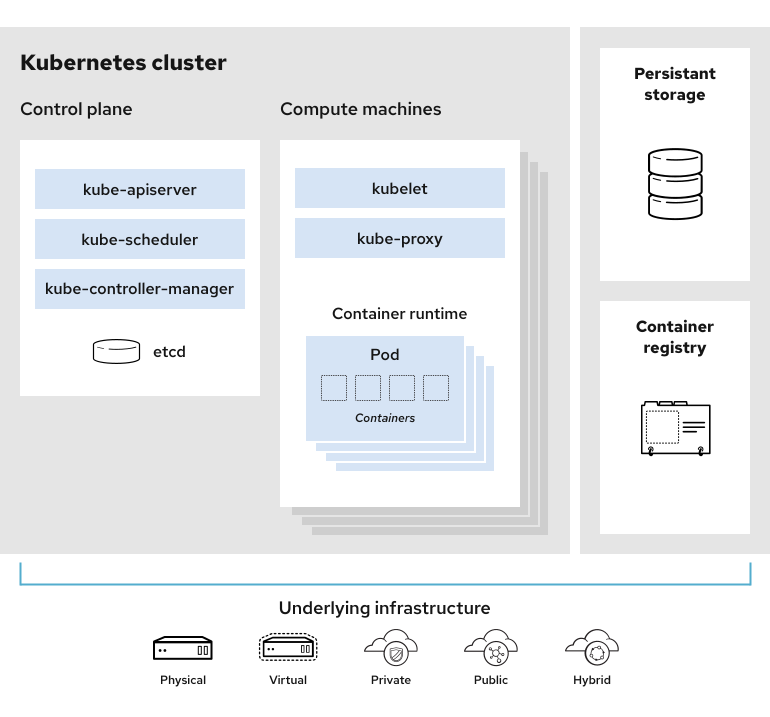
\includegraphics[width=\columnwidth]{figures/kubernetes}
\caption{The Kubernetes architecture \label{fig:kubernetes}. Source \cite{k8s-architecture}.}
\end{figure}

Kubernetes \cite{kubernetes} is a open-source framework designed to manage containerized workloads on clusters and originated from Google's experience with cloud services. Fig. \ref{fig:kubernetes} illustrates the main components of the architecture.

The basic building block in Kubernetes is a Pod. A Pod encapsulates one or more tightly coupled containers that are colocated and share the same set of resources. Pods also encapsulate storage resources, a network IP, and a set of options that govern how the Pod's container(s) should run. A Pod is designed to run a single instance of an application enabling horizontal scaling by replicating multiple Pods across the nodes. The amount of CPU, memory, and ephemeral storage a container needs can be specified when creating a Pod. This information can then be used to make decisions on Pod placement. These compute resources can be specified both as a requested amount or a as cap on the amount the container is allowed to consume. \textcolor{blue}{TODO: expand architecture overview}

From a technical perspective, Kubernetes allows for various types of container runtimes to be used, with Docker natively supported by the platform. Thanks to the standardisation of the Container Runtime Interface (CRI) API, Kubernetes supports other container technologies such as containerd \cite{containerd} or Firecracker and gVisor mentioned before. Moreover, etcd \cite{etcd} is an open-source highly available distributed key value store and a fundamental part in supporting Kubernetes in the management of the cluster nodes and jobs. Specifically, etcd is used to store all of the cluster's data and acts as the single source of truth for all of the framework's components.

Overall, Kubernetes is a highly mature system; it stemmed from 10 years of experience at Google and it is the leading container-based cluster management system with an extensive community-driven support and development base. It provides users with a wide range of options for managing their Pods and the way in which they are scheduled, even allowing for pluggable customised schedulers to be easily integrated into the system.

Besides the extensible scheduler, which makes Kubernetes already an intriguing choice as a potential orchestrator for the continuum, it also supports label-based constraints for the Pods' deployment. Developers can define their own labels to specify identifying attributes of objects that are meaningful and relevant to them, but that do not reflect the characteristics or semantics of the system directly. An example, it would allow to specify that a IoT device component must be reachable from the host or a persistent storage available, e.g. a Solid State Drive. But more importantly, labels can be used as well to force the scheduler to colocate services that communicate a lot into the same availability zone, improving drastically the latency and paving the way for context-aware services. To realize the heterogeneity goals however, it is required to continuously filter unqualified resources and new resource affinity models should be proposed to rank the resources when provisioning for different applications. 

Finally, Kubernetes is also designed with multitenancy in mind, compared to Docker Swarm \cite{docker-swarm}, which is another popular open-source orchestrator often cited as main competitor for edge orchestration due to its simplicity (e.g. \cite{containers-fog} and \cite{docker-edge-computing}). Support for multitenancy is a must and well aligned with their goal of executing heterogeneous services on a set of shared resources.

\subsubsection{Akri}
\label{sec:akri}

\begin{figure}[h]
\centering
\includegraphics[width=\columnwidth]{figures/akri}
\caption{The Akri architecture \label{fig:akri}}
\end{figure}

Akri \cite{akri} is an open-source project which extends the Kubernetes Device Plugins API \cite{k8s-device-plugins} to allow visibility to IoT devices from applications running within the cluster. The Device Plugin API is originally designed to expose hardware resources attached to a kubelet, such as GPUs or Solid State Drives, and it is still at the experimental stage. Akri stretched the design further so that it would be possible to implement discovery of IoT devices, with support for the diversity of communication protocols and the ephemeral availabilities.

Akri's architecture, presented in Fig. \ref{fig:akri}, can be divided into four main component: the agents, the controller, the brokers and the configuration. A configuration is a Kubernetes Custom Resource Definition (CRD) to extend the Kubernetes api with new types of resources. Specifically, a configuration defines a communication protocol (e.g. OPC UA \cite{rest-opc}) and the related metadata, such as the protocol discovery parameters or the Docker image to use as agent.

The Akri agent is a Pod responsible for discovering devices according to a communication protocol and can be easily developed and deployed to the cluster to support new protocols in the system. The agent will track the state of the device and keep the Akri controller updated with the status. At the time of writing, the project has built-in support for ONVIF \cite{onvif}, udev \cite{udev} and OCP UA \cite{rest-opc} discovery handlers, with an incoming proposal for CoAP \cite{coap} written by this thesis' author.

By using Akri, the Kubernetes cluster is able to carry out dynamic discovery to make use of new resources as they become available, as well as move away from decommissioned/failed resources. Discovering IoT devices is usually accomplished by scanning all connected communication interfaces and enlisting all locally available resources.

Lastly, the Akri controller advertises discovered leaf devices to the Kubernetes resources manager, making them visible to any application that requires IoT devices to work. The controller is also responsible for enabling applications to communicate with the device as well, by deploying a broker Pod as intermediary. 

The broker is any application instructed to communicate with the device, but Akri doesn't put any kind of constraint. As an example, Akri could be configured to deploy a broker that exposes a gRPC \cite{gRPC} interface and translate the requests to the underlying IoT communication protocol. In this thesis' view, the broker should be a web server that abstracts the actual communication between devices and applications behind a RESTful API. Such perspective is in line with the reasons presented before to choose the REST architecture as uniform interface for services in the continuum. Akri should automatically find all the devices in the environment and make them available as web resources. As an instance, the agent discovers the devices on a regular basis by scanning for CoAP (Section §\ref{sec:coap}) resources.

Besides, the broker could offer local aggregates of device-level services. For example, it can offer a service that returns the combined temperature measurements of all the things connected to it at any given time.

A RESTful broker can also help to scale with the number of concurrent HTTP requests by implementing highly performant cache mechanisms. The IoT resource periodically sends its sensor readings to the broker, where the values are cached locally. Each application request is then served directly from this cache without accessing the actual device, improving the average roundtrip time.

The broker architecture has also the advantage of fully decoupling the leaf node from the cluster workload, as it only needs to send an update packet with a frequency short enough to ensure the validity of data. On the other hand, the staleness of the retrieved data will depend on the frequency of updates sent by the device. Forwarding the HTTP request (properly translated) has instead the advantage of returning always the most recent sensor reading when the request is processed. Obviously, the cache mechanism cannot be applied for non-cacheable requests (e.g. HTTP POST) that must be sent to devices, such as turning on LEDs or changing application state.

As many distributed monitoring applications are usually read-only during their operation (e.g. sensors collecting data), this architecture exhibits a greater scalability level. A potential goal is to enables new types of services where physical sensors can be shared with thousands of users with little, if any, impact on the latency and data staleness. A representative of such case is tracking public transportation with sub-second accuracy \cite{urllc}.

\subsection{CoAP}
\label{sec:coap}

\begin{figure}[h]
\centering
\includegraphics[width=\columnwidth]{figures/coap}
\caption{The REST architecture enhanced with CoAP \label{fig:coap}. Source \cite{coap}.}
\end{figure}

CoAP \cite{coap} (RFC 7252) is a web communication protocol for use with constrained nodes and constrained (e.g. low-power, lossy) networks. The protocol is designed for M2M applications and provides a client-server architecture between IoT nodes, but supports built-in discovery of resources as well.

A central element of CoAP's reduced complexity is that, instead of TCP, it uses the UDP transport protocol and defines a very simple message layer for retransmitting lost packets. The rationale for UDP is that TCP carries significant overhead and can have suboptimal performance for links with high packet loss, both of which are common across the Internet \cite{akamai} and especially on remote locations where sensors might be deployed. Besides, the HTTP protocol adds further burden, as the additionally multiple round trips required for the requests can quickly add up, affecting the device performance and energy efficiency.

Within UDP packets, CoAP uses a four-bytes binary header, followed by a sequence of options, each up to two bytes. The protocol's specification also defines the familiar four request methods: GET, PUT, POST, and DELETE. Similarly, response codes are patterned after the HTTP response codes.

The protocol is built upon key concepts of the web such as URIs and RESTful interaction \cite{coap-soa}. As result, CoAP easily interfaces with HTTP for integration with web services while meeting specialized IoT requirements such as multicast support, very low overhead and simplicity for constrained environments. 

The URI format allows exposing device data as resources and the use of standard and specialized service endpoints. For instance, CoAP servers are encouraged to provide resource descriptions available via the well-known URI \emph{/.well-known/core} to achieve resource discovery. Clients then access this description with a GET request on that URI, usually via a IPv4 or IPv6 broadcast message. The description format is based on the CoRE Link format (RFC 6690), which is simple and easy to parse. Ease of parsing allows more efficient M2M discovery and inter-communication between the nodes themselves.

The CoAP protocol allows to support different resource representations, in line with the representation negotation advocated by the REST architecture. The default format is textual for its convenience when reading and parsing. The binary format is efficient to communicate, but requires external tools to make it readable by human users. XML is understandable and very well structured, but the size of its messages is big and it is much worse to parse compared to binary formats. Lastly, JSON is understandable, well structured and compact, but may still put unnecessary parsing burden on the limited device. With all constrained devices, the flash or memory consumption is one of the biggest problems, notably on devices where network connectivity already claims significant buffer memory.

Another advantage of CoAP is that, by using standard web technologies, the human interactions follow a familiar and intuitive pattern already used by many developers and thus the learning curve is smoother. This feature cannot be understimated as allowing developers to use a familiar and seamless programming experience is essential to achieve the success of the continuum.

Interoperability with the rest of the continuum can be achieved by following the REST architecture's proxy pattern, as depicted in Fig. \ref{fig:coap}. We can generally build intermediaries that speak CoAP on one side and HTTP on the other without encoding specific application knowledge. This allows deploying new applications, without having to upgrade the intermediaries involved. On the other hand, an intermediary can perform the translation between CoAP and HTTP without posing further requirements either on the client or server. Because equivalent methods, response codes, and options are present in both HTTP and CoAP protocols, the mapping between the two is straightforward. As result, an intermediary (e.g. an Akri broker) can discover CoAP resources and make them available at regular HTTP URIs, enabling web services to access CoAP servers transparently.

However, the HTTP client-initiated interaction model may be unsuited for many event-based and streaming systems in the IoT, where data is sent asynchronously to the clients as soon as it is produced. To overcome this issue, CoAP uses the Observe approach (RFC 7641) to support pushing information from servers to clients. In a GET request, a client can indicate its interest in further updates from a resource by specifying the "Observe" option. If the server accepts this option, the client becomes an observer of this resource and receives an asynchronous notification message each time it changes. This kind of communication, combined with an intermediary broker, allows streaming data updates via WebSocket (RFC 6455) and overcoming the client-pull interaction model of HTTP. The broker can also help achieving a more reliable communication by transparently changing the underlying sensor in case of unavailability or by just avoiding closing the connection in case of temporary loss of connectivity.

\subsection{WebAssembly}
\label{sec:webassembly}

\textcolor{blue}{TODO: Wasm stack machine figure}

\textcolor{blue}{TODO: Wasm portability figure}

WebAssembly (Wasm) \cite{wasm}, first announced in 2015 and released as a Minimum Viable Product in 2017, is a nascent technology that provides a strong memory isolation (through sandboxing) at near-native performance with a much smaller memory footprint. WebAssembly is language designed to addresses the problem of safe, fast, portable low-level code on the web. The project is developed by the World Wide web Consortium (W3C) with support from all major web browser vendors (Mozilla, Google, Microsoft, and Apple), thus increasing the likelihood that it will avoid serving the purposes of a single entity (e.g. Java and .NET). Developers who wish to leverage WebAssembly may write their code in a higher-level (compared to bytecode) language such as C++ or Rust and compile to a portable binary which runs on a stack-based virtual machine. Even though WebAssembly technically is a binary code format, it can be presented as a language with syntax and structure. This was an intentional design choice which makes it easier to explain and understand, without compromising compactness or ease of decoding.

A Wasm binary takes the form of one or more modules. It contains definitions for functions, globals, tables, and memories. The computation is based on a stack machine: code for a function consists of a sequence of instructions that manipulate values on an implicit operand stack, popping argument values and pushing result values. However, WebAssembly represents control flow differently from most stack machines. It does not offer simple jumps but instead provides Structured Control Flow (SCF) constructs more akin to a programming language. This ensures by construction that control flow cannot contain arbitrary branches. The SCF allows WebAssembly code to be validated and compiled in a single pass as well. SCF can also disassembled to a WebAssembly text format (.wat) that is easier to read, an often overlooked but important human factor on the web.

The memory of a WebAssembly program is a large array of bytes referred to as a linear memory or simply memory. All memory access is dynamically checked against the memory size and out of bounds access results in a trap. Linear memory is disjoint from code space, the execution stack, and the engine's data structures. Each Wasm memory access addresses linear memory at an offset from the base, $n$, of the linear memory. Thus, there is some amount of address virtualisation as an address $b$ in the sandbox is located at $b + n$ in physical memory. The Wasm runtime is responsible for translating linear memory accesses, and bounds-checking them to prevent accesses outside the sandbox.

Therefore, compiled programs cannot corrupt their execution environment, jump to arbitrary locations, or perform other undefined behaviour, especially when the original language is memory-safe (e.g. Rust §\ref{sec:rust}). At worst, a buggy or exploited WebAssembly program can make a mess of the data in its own memory.

This memory and state encapsulation is applied at module level rather than at application level, meaning that memory and functions of a module cannot leak information unless explicitly exported/returned. This granularity in sandboxing is extremely important as security incidents have been increasingly exploiting vulnerabilities in the dependency chain, as reuse of third-party software is pervasive in modern languages like JavaScript, Rust or Go. As an example, JavaScript (and consequently TypeScript \cite{typescript}) strongly relies on its package manager NPM and the latter has been increasingly subject to security incidents in the recent years \cite{npm-security}.

This means that even untrusted modules can be safely executed in the same address space as other code. Additionally, it allows a WebAssembly engine to be embedded into any other language runtime without violating memory safety, as well as enabling programs with many independent instances to exist in the same process. These sandboxing features make WebAssembly a compelling technology upon which to implement a virtualisation stack for the continuum. On the web, the substrate of the continuum, code is fetched from untrusted sources and it's vital that such code can be safely executed.

Another important safety feature of Wasm is the type system. Code must be validated before it can be executed safely. Validation rules for WebAssembly are defined succinctly as a type system. This type system is, by design, simple. It is designed to be efficiently checkable in a single linear pass, to allow parallelisable binary decoding and compilation. Moreover, function pointers cannot be dereferenced directly. A call to a function pointer is translated into an activation of a function in a runtime table of valid entry points and types. The type of the function is checked dynamically against the expected type in the said entry. The dynamic signature check protects integrity of the execution environment. In case of a type mismatch or an out of bounds table access, a trap occurs.

With that being said, the design goals of WebAssembly strongly advocate for its suitability for this thesis: \textcolor{blue}{TODO: explain why each design goal is important for the continuum}

\begin{itemize}
    \item \emph{Safe to execute}: protection for arbitrary code has traditionally been achieved by providing a managed language runtime that enforces memory safety, preventing programs from compromising user data or system state. However, managed language runtimes have traditionally not offered much for portable low-level code, such as C/C++ applications, that do not need garbage collection;
    \item \emph{Fast to execute}: low-level code like that emitted by a C/C++ compiler is typically optimized ahead-of-time. On the contrary, managed runtimes and sandboxing techniques have typically imposed a steep performance overhead on low-level code. WebAssembly is, however, very competitive with native code and benchmarks using Wasm runtimes on modern browsers have shown slowdown within 10\% compared to native execution and almost always within 2x \cite{wasm};
    \item \emph{Language, hardware, and platform independency}: as mentioned before, the web spans not only many device classes, but different machine architectures, operating systems, and browsers. Code targeting the web must therefore be independent from any underlying hardware or platform to allow applications to run across all software and hardware types with the same behaviour;
    \item \emph{Deterministic and easy to reason about}: WebAssembly has been designed with a formal semantics from the start, for both execution and validation, including a proof of soundness. Besides, the Wasm binary can be compiled into a .wat file to simplify learning and debugging;
    \item \emph{Simple interoperability}: WebAssembly is similar to a virtual ISA in that it does not define how programs are loaded into the execution engine or how they perform I/O. The embedder (i.e. the host runtime) defines how modules are loaded, how imports and exports between modules are resolved, provides foreign functions to accomplish I/O, and specifies how traps are handled. It is possible, by design, to link multiple modules that have been created by different authors, from likewise different source languages. However, as a low-level language, WebAssembly does not provide any built-in object model. It is up to developers to map their data types to numbers or the memory. This design is supposed to provide maximum flexibility to developers, and unlike previous VMs like Java or .NET, does not privilege any specific programming or object model while penalizing others. The downside of this design is that interoperability with object references is cumbersome when it involves exchanging references between the Wasm application and the host code or between modules originated from different languages. A step in easing this issue is the recent introduction of Reference Types \cite{reference-types}. On the other hand, since WebAssembly is an abstraction over hardware, not over a programming language, a WebAssembly module may be compiled once and moved freely between different hardware architectures with no recompilation;
    \item \emph{Compact}: the binary code is designed to be compact, especially compared to bytecode in text format. For this reason, it is recommended distributing the binary code on the Internet code and using the text format only for learning and debugging. Code transmitted over the network has to be as compact as possible to reduce load times, save potentially expensive bandwidth, reduce memory usage on constrained network-attached devices and improve overall responsiveness;
    \item \emph{Easy to validate and compile}: validation proceeds by checking on-the-fly while the incoming bytecodes are arriving, with no intermediate representation (IR) being constructed. Benchmarks run on mainstream browsers in \cite{wasm} prove that validation can be fast enough be performed at full network speed of 1Gib/s;
    \item \emph{Streamable and parallelisable}: a Wasm runtime can minimize latency by starting streaming compilation as soon as function bodies arrive over the network. It can also parallelize compilation of consecutive function bodies. For instance, each function body is preceded by its size so that a decoder can skip ahead and parallelize even its decoding.
\end{itemize}

Despite the name WebAssembly, there has been a significant effort in the last years in adopting Wasm for a native execution, as it is a portable target for compilation of various high-level languages. Wasm standard does not necessarily make browser-specific assumptions and there has been substantial work to standardize the WebAssembly System Interface (WASI) to run Wasm outside the browser. To the best of the author's knowledge, the original design goals assumed a browser-based execution context. Nevertheless, such goals fit perfectly to the needs of the continuum, where the web is the infrastructure upon which applications and services are deployed. On this matter, browsers are very much akin to an Operative System for client web applications and WebAssembly is thus unsurprisingly being adopted on conventional OSes. Native execution and browser execution share many problems, like isolation, portability and interoperability to name just a few.

At the time of writing, there are a number of Wasm runtimes for programs written in different languages to embed Wasm applications. At same time there are different compilers which can compile languages to Wasm, notably the Wasm back-end for LLVM \cite{llvm} works for C, C++, and Rust. Commercial solutions have also been slowly but steadily gaining popularity. Cloudflare's Service Workers \cite{cloudflare-workers} began to offer support for creating and hosting serverless functions in WebAssembly. In March 2019, the edge-computing platform Fastly has announced and open-sourced Lucet \cite{fastly-lucet} that provides a compiler and runtime to enable native execution of Wasm applications and can instantiate a Wasm module within $50\mu s$, with just a few kilobytes of memory overhead. Parity is also actively experimenting with writing smart contracts using Wasm \cite{parity-wasm}.

Because of its design features, WebAssembly is currently under experimentation as a new method for running portable applications without the use of containers. This method leverages its binary format a portable vehicle to inherent memory and execution safety guarantees via its language features and a runtime with strong sandboxing capabilities. The Wasm security model enables execution of multiple untrusted modules in the same process, thereby providing significantly more lightweight isolation compared to VMs and containers for multi-tenant serverless execution \cite{sledge}.

This idea is still at its infancy but there has been some interest in the recent years, as shown by the works done in \cite{execution-model-serverless-edge} and \cite{faasm}. All these works focus primarly on serverless computing via WebAssembly, a demonstration of the gain in popularity of such computing model. As this thesis have stated before however, if serverless were the only execution model, it would severley limit the variety of applications in the continuum.

\subsubsection{Krustlet}

\textcolor{blue}{TODO}

The current WebAssembly System Interface (WASI) standard only contains a few methods for working with sockets, namely \emph{sock\_recv}, \emph{sock\_send}, and \emph{sock\_shutdown}, that are not enough for complete networking support. Adding support for connecting to sockets is fundamental to allow Wasm modules to connect to web servers, databases, or any service.

\subsubsection{WebAssembly for embedded microcontrollers}

An emerging use case for WebAssembly is arbitrary code execution on microcontrollers and, as result, interpreters are gaining popularity on resource-limited devices. wasm3 \cite{wasm3} is a popular open-source interpreter capable of running on any system with at least 64KiB of storage and 10KiB of memory. The authors of eWASM \cite{ewasm} have also explored various mechanisms for memory bounds checking and have evaluated the trade-offs between processing efficiency and memory consumption. Just-In-Time compilers for WebAssembly exist (e.g. Wasmtime \cite{wasmtime}) and receive more attention from the community, but their size and complexity make them unsuitable for microcontrollers.

Although, WebAssembly interpreters can often be approximately 11x slower than native C \cite{wasm3-performance}, they are useful for dynamically updating system code and debugging, but may not be applicable for code on devices extremely sensitive to performance and energy efficiency.

In the author's view, interpreting WebAssembly on microcontrollers remains an intriguing technology nevertheless, worth the attention of the research community. They offer a persuasive alternative to other language runtimes, e.g. Lua, which are commonly used on embedded devices to support dynamic configuration \cite{levee}. The WebAssembly standard has a number of features that make it appealing for embedded devices \cite{ewasm}.

\begin{itemize}
    \item Broad support: there is a steadily increasingly ecosystem of vendors, tools, and languages providing WebAssembly support. With the ability to leverage WebAssembly, the embedded system community would benefit from a broader ecosystem;
    \item Portability: WebAssembly is a platform-independent Intermediate Representation that can be generated from different source languages, and can run on many CPU architectures. Solving how to effectively run WebAssembly on microcontrollers would open the possibility to include the embedded world to the continuum as additional place of intelligent computing, rather than only as mere data collector and dummy actuator;
    \item No mandatory garbage collection. Many broadly used language runtimes such as JavaScript, lua, or python cannot provide predictable execution and may require excessive memory for a microcontroller;
    \item Lightweight runtime: WebAssembly mandates only a small number of runtime features around maintaining memory sandboxing. These light requirements help in an embedded adaptation.
\end{itemize}

\subsection{Rust}
\label{sec:rust}

As the continuum integrates computing throughout the network, the attack surface greatly increases consequently. Security has to be a top priority during software development, yet most of the infrastructure is programmed using the C, C++ programming languages. These two programming languages are chosen due to the low overhead on memory and the high processing performance. Embedded systems has favoured the two languages because of the need for low level control over the hardware.  However, C and C++ are not particularly known for producing secure software as evidenced by the large number of vulnerabilities reported against software written in them. Notably, the main cause of security vulnerabilities are memory safety bugs like data races and buffer overflows. Even higher-level languages suffer from these kinds of safety issues. The Go language, upon which most of the modern distributed systems are built (namely Kubernetes), is not exempt from exploits based on data races \cite{go-data-races}.

On the other hand, Rust is a strongly-typed, compiled language that uses a lightweight runtime similar to C. Unlike many other modern languages, Rust is an attractive choice for predictable performance because it does not use a garbage collector. It provides strong memory safety guarantees by focusing on "zero-cost abstractions", meaning that safety checks are done at compile time and runtime checks (e.g. out-of-bounds access) have the minimum overhead and come with a predictable cost.

Not all operations can be verified to be memory safe at compile time. One example is indexing a slice, a partial view into an array. In this case, the indexing operation contains a runtime check to check if the index is within bounds. If the index is out of bounds then the result is a panic. A panicking condition can result in either aborting the whole program or just unwinding the stack of the thread that ran into the panic. The unwinding process walks up the stack freeing all live resources before terminating the thread, ensuring a clean memory state afterwards.

In the Rust community, there is strong emphasis on building safe abstractions with almost zero runtime cost. Safe Rust code is guaranteed to be free of null or dangling pointer dereferences, invalid variable values (e.g. casts are checked), reads from uninitialized memory, unsafe mutations of shared data, and data races, among other misbehaviours.  The borrow checker, the most innovative feature of the language compiler, runs as part of the compilation process and catches bugs like just mentioned misbehaviours. Security cannot be achieved without memory safety so it is fundamental that the latter is a property of the language and not a concern of the developer only.

% The main four aspects of the Rust memory safety are:

% \begin{itemize}
%     \item Ownership: the compiler tracks the lifetime of resources, like memory allocations, through variable assignments and function calls. A resource assigned to a variable is said to be owned by the variable. Passing a variable to a function causes the ownership of the resource to be transferred to the callee; this operation in known as a move in Rust terminology. After moving the resource out of a variable the variable can no longer be used to access the resource. When a variable goes out of scope the resource it owns is freed, i.e. the destructor is called;
%     \item References: when a move is not desired, borrowing can be used. Borrowing a value creates a reference to it. References in Rust are pointers that are guaranteed to be valid at compile time. References are never null and always point to a live and valid memory location. To cope with the problem of unsynchronized mutation the Rust programming languages provides two kinds of references: immutable references and mutable references. At any time, the language allows many immutable references to the same memory location \emph{or} a single mutable reference to exist;
%     \item Lifetime: the compiler uses lifetimes to track the liveness of variables. The borrow checkers checks that borrows do not outlive (have a span longer than) the lifetime of the data they refer to;
%     \item Concurrency: Rust provides two marker traits in the core library that are used to build concurrency primitives: Send and Sync. Send types can be transferred across thread boundaries, whereas Sync types are safe to share references between threads. Values are required to implement these traits to be accesses concurrently. Concurrent access is not limited neither to two or more cores accessing the value in parallel. Single core runtimes can likewise access a value concurrently. Examples of the latter scenario include POSIX signal handlers on a single-core system, time-sliced threads running on a single-core system, and interrupt handlers on a embedded system.
% \end{itemize}

In the author's view, Rust is a strongly recommended choice as the implementation language for the infrastructure of the continuum. Rust is one of the few alternatives to C and C++ that can equally compete in terms of performance, low-level control and cross-platform support. Its use cases are not limited to system development though. Although initially advertised as a system language, Rust is nowadays dedscribed as a language to build any reliable and performant software. Use cases ranges from embedded systems and Operative Systems to web servers and user interfaces (e.g. via WebAssembly on the browser). Thanks to its vast community of open-source libraries and productivity tools, it can be a sensible alternative even for high-level services.

Its toolchain is backed by the LLVM modular compiler infrastructure, which Rust relies on for translating high-level code from languages such as C++ to its own intermediate representation (IR). In addition to code translation, LLVM also provides several tools which aid in tasks such as optimisation and dead code elimination. Thanks to the integration of LLVM, the Rust compiler rustc can transform this IR to generate WebAssembly binary code as well. The union of Rust and WebAssembly constitutes a powerful combination. Developers can write source code in Rust to achieve high productivity and efficient memory-safe applications. On the other hand, WebAssembly can contribute with universal portability of such binaries without compiling or distributing multiple versions (e.g. Docker image versions). 

\subsubsection{RTIC}

Rust is gaining popularity as language for embedded systems as well. The language provides a rich standard library, which relies however on dynamic memory allocation provided by the host operating system, not available on embedded devices. Fortunately, the standard library is built on a core library, that neither requires dynamic allocations nor any host operating system. These minimal dependencies make it possible for Rust applications to be built and executed on bare metal targets. Likewise, many Rust libraries that may be needed on embedded environments come with support for "no\_std", i.e. the library can be compiled without the standard library. 

The Rust compiler rustc supports a wide range of platforms and architectures as well. Passing a compilation target to rustc allows to compile the source code to machine code optimized for the target platform.

A further step towards the maturity of Rust as language for embedded systems is the framework Real-Time Interrupt-driven Concurrency (RTIC) \cite{rtic}, previously known as Real-Time For the Masses (RTFM) \cite{rtfm}. RTIC is a framework developed by the Embedded Systems group at the Luleå University of Technology (LTU) for leveraging the interrupt controller (shortly explained) to schedule tasks of different priority, while the risk of deadlock is mitigated thanks to all resource-accesses being handled by the Stack Resource Policy (SRP) \cite{stack-resource-policy}.

Stack Resource Policy is a method to handle resource access in real-time systems with a single shared stack. RTIC uses SRP to handle access to resources and it guarantees a race and deadlock-free preemptive execution, along with bounded priority inversion. Additionally, the model does not use excessive memory for the stack since the tasks all share common stack space.

RTIC implements the SRP using hardware interrupts. An interrupt signal is a hardware-generated event that usually occurs asynchronously with respect to the execution of the program. Examples of signals include an electrical pin changing its logical state from 0 to 1 or vice versa, a timer reaching a certain value, or data becoming available on some communication interface. In response to these signals the processor executes an interrupt handler, a special subroutine. Interrupts have also an associated priority level. In the case of the ARM Cortex-M architecture all interrupts have higher priority than the thread mode, reserved for the common procedures, so handlers will preempt code running in thread mode.

Preemption works as follows: the processor suspends the execution of the current subroutine, saves the state of that subroutine (the processor registers) onto the stack and then jumps to the interrupt handler. The interrupt handler runs to completion and returns. Upon returning from the interrupt handler the state of the suspended routine is restored by popping the registers off the stack and the preempted routine is resumed.

All these interrupts are managed by the Nested Vector Interrupt Controller (NVIC) peripheral \cite{definitive-guide-cortex}. The NVIC is a standardized interrupt controller found on all Cortex-M devices. The NVIC provides an interface to control and configure interrupts in the form of memory mapped registers.

The way the NVIC handles interrupts \cite{interrupts-handling} exactly matches how the RTIC task model prioritizes tasks. This fact is used to provide a highly efficient implementation: the RTIC runtime lets the NVIC, the hardware, do all the task scheduling so no book-keeping needs to be done in software. The priority of the task is thus bound to the interrupt service routine (ISR) matching that priority, associating an ISR to each interrupt handler, represented by a task. This alternative to time sliced threads provides several advantages like reduced overhead, efficient memory utilization, predictable performance (constant time overhead), deadlock freedom and suitability for static analysis \cite{rtfm}.

\subsection{Architecture}

Having presented the technology background, the architecture of this thesis is now presented. To the best of the author's knowledge, this thesis is the first of kind which tries to combine the vision of the computing continuum and the proposal of a technology baseline, whose sensibility is demonstrated with a Proof of Concept (POC). Notably, the goal of the POC is to prove that the technologies mentioned above can be integrated together to support the realisation of the continuum's infrastructure layer. 

The infrastructure layer is composed of data and computational resources. The data can be generated by various streaming IoT devices (e.g. cameras, smart watches, and smart infrastructure). The computational resources can be heterogeneous and distributed through the infrastructure, from the cloud to the edges.

In order to support a truly ubiquitous system where services are everywhere and anywhere the end-user is, for instance following the movements across geographical zones, further architectural considerations have to be made. As an example, a federation layer may fit as solution. The federation layer would responsible for orchestrating the geographically distributed resources composing the underlying infrastructure. However, this thesis will not explore such federation layer and it is left as open research question of future works on the continuum.

\begin{figure}[h]
\centering
\includegraphics[width=\columnwidth]{figures/architecture}
\caption{Reference architecture \label{fig:architecture}}
\end{figure}

With the goal being said, a reference architecture of the infrastructure is shown in Fig. \ref{fig:architecture}. From a high-level perspective, users submit applications to the orchestrator. The orchestrator provisions the necessary resources and services according to the requirements indicated by the application, then assigns the latter to compute nodes in the cluster, where they are executed. The compute cluster is an abstraction of interconnected nodes that can be on geographically distant clusters, such as clouds and fog nodes.

Users submit their applications in the form of a manifest. The manifest describes resources requirements in terms of the amount of CPU and memory they will require for example. Likewise, the manifest contains the service requirements as well. Services may range from common dependencies like a database and a persistant storage to data sources, which the cluster will take care to provide based on the stated requirements. Service requirements allow developers to describe contraints on the services, e.g. latency needs and service plans. Unfortunately, as of time of writing, this thesis has not explored standard manifest formats to describe such service requirements. The POC merely leverages the Kubernetes YAML format, which specifies information like the container image, the placement constraints, and the resource requests.

\subsubsection{Orchestrator control plane}

The Kubernetes control plane is the core of the orchestration system. It has a resource monitor module responsible for keeping track of real-time resource consumption metrics for each node in the compute cluster. This information is usually accessed by the scheduler to make better optimisation decisions. The scheduler is responsible for determining whether there are enough resources and services available in the continuum to execute the submitted application. In case resources are insufficient, applications can be rejected or put on wait until the resources are freed. Another possible solution would be to increase the number of cluster nodes to place the incoming application. Such nodes may be provisioned from local machines or anywhere in the network path from the end-user to the cloud datacentre. After determing if requirements can be satisfied, the scheduler maps application components, or more specifically Kubernetes Pods, onto the cluster resources. This is done by considering several factors, e.g. the availabilities, the utilization of the nodes, affinities, priorities, or constraints.

In cases where the addition of new cluster nodes is possible, an automatic process is necessary. The provisioner is responsible for dynamically adding nodes (physical or virtual) to the cluster when the existing resources are insufficient to meet the applications' demands. It will also decide when nodes are no longer required in the cluster and will shut the nodes down to prevent incurring in additional costs.

\subsubsection{Compute nodes}

Each machine in the cluster that is available for deploying Pods is a compute node. Each of these nodes has an implementation of the Kubelet APIs with various responsibilities. First, it collects local information such as resource consumption metrics that can be periodically reported to the control plane. Second, it starts and stops Pods and manages local resources, via a container runtime or a Wasm runtime. Finally, it monitors the Pods deployed on the node, sending periodic status to the control plane.

The reason for the presence of two types of compute nodes lies in the lack of maturity of the Wasm ecosystem at the time of writing. As previously mentioned, Krustlet is still far from reaching feature parity compared to a standard Kubelet implementation. As an example, support for the Kubernetes networking is not implemented yet, nor machine metrics are collected and sent to the control plane. Besides, as stated before, the current WebAssembly System Interface (WASI) standard doesn't have a complete networking support yet. Adding support for connecting to sockets is fundamental to allow Wasm modules to connect to web servers, databases, or any service. Because of the lack of network support, both as API in the Wasm module and as network configuration in the Kubernetes cluster, the POC uses a hybrid approach where conventional kubelets with container runtimes are used as fallback.

\subsubsection{IoT nodes}

IoT nodes are embedded devices that act as sensors and actuators, provided as service to the cluster. The IoT nodes are heterogeneous in runtime implementation and communication protocols, therefore applications in the cluster interface with the them via Akri brokers as described before. However, in the POC of this thesis, embedded devices use the RTIC runtime implemented in Rust and support dynamic configuration by running arbitrary Wasm modules in a lightweight Wasm runtime.

The Wasm runtime is implemented via an interpreter capable of executing any regular Wasm binary, assuming the file size and the hardware requirements can be satisfied by the limited device.

\subsubsection{Underlying infrastructure}

One of the main benefits of containers is their flexibility in being deployed in a multitude of platforms. Because of these, the cluster machines can be either VMs on public or private cloud infrastructures, physical machines on a cluster, or even mobile or edge devices among others.

\section{Evaluation}
\label{sec:evaluation}

% First, we evaluate our Sledge compiler aWsm and runtime on x86\_64 and AArch64 architectures using two systems:

% \begin{itemize}
%     \item MacBook Pro 15" 2018 with 6-Core Intel Core i7 2,2GHz and 16GB of RAM;
%     \item Raspberry Pi 4 Model 3B+ with Quad-core Cortex-A53 (ARMv8) 64-bit SoC at 1.4GHz and 4 GB physical memory.
% \end{itemize}

% Sensor networks represent a crucial component in IoT environments \cite{edge-computing-survey}. For example, they can cooperate with RFID systems to better track things, get information about the position, movement, temperature, etc. Sensor networks are typically composed of a potentially high number of sensing nodes, communicating in a wireless multi-hop fashion.

% Wireless sensor networks (WSNs) can provide various valuable data and are being utilised in several areas like healthcare, government and environmental services (natural disaster relief), defence (military target tracking and surveillance), hazardous environment exploration, seismic sensing, etc.

% Recent technological advances have made efficient, low-cost, and low-power miniaturised devices available for large-scale remote sensing applications. In this context, the timely processing of massive and streaming sensor data, subject to energy and network constraints and uncertainties, has been identified as the main challenge.

% \subsection{Kubernetes}

% - OSB is not meant for machines (M2M)
% - The Device Plugin APIs is meant for hardware attached to a node, not for advertising edge nodes

% \subsection{Web Assembly}

% The startup latency for initiating a function instance in a FaaS platform can vary significantly: from a few milliseconds to several seconds. A function execution might be a “warm-start", reusing a VM or container from the previous event of the same function, or it might be a “cold-start", where a new VM/container has to be launched.

% Application developers employ work-arounds to avoid startup delays, including artificially activating functions (to avoid container shutdown) or over-provisioning resources required to run their functions. On a container-based serverless computing platform in an edge computing environment, containers that are long-lived or overprovisioned can quickly degrade performance due to limited available resources. Setup and control of these features requires multiple syscalls and IPC between container parent and child processes before a serverless function can begin executing. 

% Each Docker container consists of one or more separate processes, whereas each Wasm instance is contained within the same V8 process. This provides a Wasm-based solution the advantage of warmer caches and reduced context switch penalties, creating better potential for speedup when concurrently executing multiple serverless functions. Although in general a container's overhead may be acceptable for long-running applications, this overhead quickly proves an impediment to meeting the low-latency demands of serving emerging IoT applications.

% Wasm's primary advantage over container-based solutions is the absence of a large cold start penalty. There are two reasons for this advantage. First, container runtimes such as Docker incur a large amount of overhead in ensuring their support for containers is as broad as possible.

% The Sledge runtime decouples the heavy-weight function linking and loading process from function instantiation process.

% Many of the existing Wasm runtimes can exhibit significant overhead in properly sandboxing code.

% We must provide a way for our solution to limit an application's execution time and maximum memory usage. In container-based platforms, this resource control is achieved via the Linux control groups feature. This feature allows one or more processes to be organized into groups which have their resources monitored and limited by the kernel. Maximum Memory Usage: current runtimes rely on WebAssembly's JavaScript API to perform this memory creation operation. The WebAssembly.Memory() API function allows us to set initial and maximum sizes for the linear memory to be created. Execution Time: nope.

% The use of WebAssembly in a serverless platform should not require application developers an undue amount of work in porting their existing code to the new runtime. Currently, support for many popular programming languages (e.g., C\#, Go, Python, Java) is in active development across numerous open-source projects.

% Creating several new programs and adapting existing popular libraries for use in WebAssembly, the amount of manual work involved was minimal.

% There is an underlying issue with implementing network servers: there is no multi-threading support in WebAssembly - which means that a server running in WebAssembly is either going to be single-threaded, or its implementation would have to be significantly more complex (see Node's event loop ). At the same time, there is a WebAssembly threads proposal that would define operations for handling atomic memory access across threads, but it is only at stage 2 of the Wasm standardization process.

% \subsubsection{Wasm for microcontrollers}

% We use STM32F767ZIT6, a Cortex-M7 based microcontroller for evaluation of wasmi. It runs at 168MHz,128kB SRAM, and 5121KiB flash.

% Linear memory is dynamically sized. It is extended in increments of a 64KiB page size. 

% Running SFI on resource constrained microcontrollers presents a number of challenges.

% \begin{itemize}
%     \item Memory consumption. Wasm's 64 KiB pages are too large for microcontrollers that often have between 16-256 KiB SRAM. \cite{ewasm} implementation departs from the standard by allowing byte-granularity, 1 KiB page-granularity
%     \item Performance. Though the bounds checking on linear memory and the indirect checking of function pointer invocations are necessary for proper isolation, they add overhead over non-sandboxed code.
%     \item Assumed ISA features. Wasm specifically is a 32-bit virtual architecture and supports floating point, but not all Cortex-Ms do. In such cases, floating-point emulation is broadly deployed.
% \end{itemize}

% \subsection{Rust}

% Code generation is done via Rust macros 41 detailed in the advanced features part of the Rust book. Macros are what is known as metaprogramming, which essentially is writing code which manipulates code. 

% The downside to implementing a macro instead of a function is that macro definitions are more complex than function definitions because you're writing Rust code that writes Rust code. Due to this indirection, macro definitions are generally more difficult to read, understand, and maintain than function definitions.

% The tooling for debugging rust macros are not easy to use, even though tools like cargo-expand 42 significantly improves the situation. It produces the expanded output of the macro, meaning that the code passed to the compiler can be inspected in order to verify correct operation.

% \subsection{RTIC}

% RTFM implements best effort scheduling based on static task priorities. For static analysis under Rate Monotonic scheduling, minimum inter-arrival is assumed to be larger or equal to the deadline of the task.

% Static analysis and in particular Worst Case Execution Time (WCET) and stack usage analyses are required components of the certification process of safety critical software. Due to their age and popularity plenty of C and C++ tooling exists for static analysis: from sanitizers that find data races and memory bugs in software to static stack usage analysis tools that find the worst case stack usage of an application. Only a handful of these tools, namely sanitizers, can be used on Rust programs.

% To indicate that these pointers need special attention from the programmer the language has the concept of unsafe operations. Unsafe operations cannot be proven to be memory safe by the compiler; the programmer must manually verify that they are indeed memory safe. This makes them easy to spot and facilitates the process of auditing Rust code for memory bugs.

% When writing embedded Rust code only a subset of the standard library is available: the core library.

% One can adopt a custom allocator, e.g. heapless which is fallible by construction (allowing the user to directly face OOM upfront, thus allowing system availability to be maintained, even if the allocator runs out of resources.

% The problem that can arise with this layout is that the stack can grow too large and collide into the heap. This situation is called a stack overflow, or stack overrun.

% cargo-call-stack is a Cargo subcommand that performs whole program stack usage analysis of a Rust application and produces a DOT file that contains the call graph of the program where each node in the call graph is annotated with its individual stack usage and cumulative (worst-case) stack usage.

% if things go wrong and the documentation does not specify how things are done, many developers turn directly to the code for understanding the implementation details. As discussed previously understanding and then debugging Rust macros is one major roadblock many get dissuaded by due to the general complexity.

\section{Conclusion}
\label{sec:conclusion}

\textcolor{blue}{TODO}

\appendix 
\blankpage


\backmatter

\cleardoublepage
\begin{thebibliography}{00}

\bibitem{ericsson-5g} Ericsson Mobility Report. [Online]. Available: \url{https://www.ericsson.com/en/mobility-report}. Accessed on Apr. 15, 2021.

\bibitem{iot-manifacturing} Chen, B., Wan, J., Celesti, A., Li, D., Abbas, H. and Zhang, Q., 2018. Edge computing in IoT-based manufacturing. IEEE Communications Magazine, 56(9), pp.103-109.

\bibitem{dsu} Mugarza, I., Amurrio, A., Azketa, E. and Jacob, E., 2019. Dynamic software updates to enhance security and privacy in high availability energy management applications in smart cities. IEEE Access, 7, pp.42269-42279.

\bibitem{saaas} Mitton, N., Papavassiliou, S., Puliafito, A. and Trivedi, K.S., 2012. Combining Cloud and sensors in a smart city environment.

\bibitem{iot-definition} Whitmore, A., Agarwal, A. and Da Xu, L., 2015. The Internet of Things—A survey of topics and trends. Information systems frontiers, 17(2), pp.261-274.

\bibitem{harnessing-continuum} Beckman, P., Dongarra, J., Ferrier, N., Fox, G., Moore, T., Reed, D. and Beck, M., 2020. Harnessing the Computing Continuum for Programming Our World. Fog Computing: Theory and Practice, pp.215-230.

\bibitem{computing-in-continuum} AbdelBaky, M., Zou, M., Zamani, A.R., Renart, E., Diaz-Montes, J. and Parashar, M., 2017, June. Computing in the continuum: Combining pervasive devices and services to support data-driven applications. In 2017 IEEE 37th International Conference on Distributed Computing Systems (ICDCS) (pp. 1815-1824). IEEE.

\bibitem{iot-enterprise} Haller S., Karnouskos S., Schroth C. (2009) The Internet of Things in an Enterprise Context. In: Domingue J., Fensel D., Traverso P. (eds) Future Internet – FIS 2008. FIS 2008. Lecture Notes in Computer Science, vol 5468. Springer, Berlin, Heidelberg.

\bibitem{fluid-internet} Latre, S., Famaey, J., De Turck, F. and Demeester, P., 2014. The fluid internet: service-centric management of a virtualised future internet. IEEE Communications Magazine, 52(1), pp.140-148.

\bibitem{cloud-iot} Botta, A., De Donato, W., Persico, V. and Pescapé, A., 2016. Integration of cloud computing and internet of things: a survey. Future generation computer systems, 56, pp.684-700.

\bibitem{cloud-def} Mell, P., and Grance, T. 2011. The NIST definition of cloud computing, Recommendations of the National Istitute of Standards and Technology, NIST Special Publication 800-145.

\bibitem{cloud-computing} Zhang, Q., Cheng, L. \& Boutaba, R. Cloud computing: state-of-the-art and research challenges. J Internet Serv Appl 1, 7–18 (2010).

\bibitem{gartner-iot} Gartner. Leading the IoT. 2017. [Online]. Available: \url{https://www.gartner.com/imagesrv/books/iot/iotEbook_digital.pdf}. Accessed on Apr. 15, 2021.

\bibitem{akamai} Nygren, E., Sitaraman, R.K. and Sun, J., 2010. The akamai network: a platform for high-performance internet applications. ACM SIGOPS Operating Systems Review, 44(3), pp.2-19.

\bibitem{aws-outage} Prolonged AWS outage takes down a big chunk of the internet. 2020. [Online]. Available: \url{https://www.theverge.com/2020/11/25/21719396/amazon-web-services-aws-outage-down-internet}. Accessed on: Apr. 15, 2021.

\bibitem{edge-computing-vision-challenges} Shi, W., Cao, J., Zhang, Q., Li, Y. and Xu, L., 2016. Edge computing: Vision and challenges. IEEE internet of things journal, 3(5), pp.637-646.

\bibitem{mobile-augmented-reality} Baresi, L., Mendonça, D.F. and Garriga, M., 2017, September. Empowering low-latency applications through a serverless edge computing architecture. In European Conference on Service-Oriented and Cloud Computing (pp. 196-210). Springer, Cham.

\bibitem{fog-computing} Cisco fog computing solutions: Unleash the power of the Internet of Things. [Online]. Available: \url{https://www.cisco.com/c/dam/en\_us/solutions/trends/iot/docs/computing-solutions.pdf}. Accessed on Apr. 15, 2021.

\bibitem{camera-virtualisation} Jang, S.Y., Lee, Y., Shin, B. and Lee, D., 2018, October. Application-aware IoT camera virtualisation for video analytics edge computing. In 2018 IEEE/ACM Symposium on Edge Computing (SEC) (pp. 132-144). IEEE.

\bibitem{raspberry} Raspberry Pi. [Online]. Available: \url{https://www.raspberrypi.org/products/}. Accessed on Apr. 15, 2021.

\bibitem{cloudlet} Satyanarayanan, M., Bahl, P., Caceres, R. and Davies, N., 2009. The case for vm-based cloudlets in mobile computing. IEEE pervasive Computing, 8(4), pp.14-23.

\bibitem{nfv-5g} Yousaf, F.Z., Bredel, M., Schaller, S. and Schneider, F., 2017. NFV and SDN—Key technology enablers for 5G networks. IEEE Journal on Selected Areas in Communications, 35(11), pp.2468-2478.

\bibitem{serverless-berkeley} Jonas, E., Schleier-Smith, J., Sreekanti, V., Tsai, C.C., Khandelwal, A., Pu, Q., Shankar, V., Carreira, J., Krauth, K., Yadwadkar, N. and Gonzalez, J.E., 2019. Cloud programming simplified: A berkeley view on serverless computing. arXiv preprint arXiv:1902.03383.

\bibitem{aws-lambda-edge} AWS Lambda@Edge. [Online]. Available: \url{https://aws.amazon.com/it/lambda/edge/}. Accessed on Apr. 15, 2021.

\bibitem{aws-greengrass} AWS IoT Greengrass. [Online]. Available: \url{https://aws.amazon.com/greengrass/}. Accessed on Apr. 15, 2021.

\bibitem{azure-iot-edge} Azure IoT Edge. [Online]. Available: \url{https://azure.microsoft.com/en-us/services/iot-edge/}. Accessed on Apr. 15, 2021.

\bibitem{serverless-mec} Baresi, L., Mendonça, D.F. and Garriga, M., 2017, September. Empowering low-latency applications through a serverless edge computing architecture. In European Conference on Service-Oriented and Cloud Computing (pp. 196-210). Springer, Cham.

\bibitem{oasis} MacKenzie, C.M., Laskey, K., McCabe, F., Brown, P.F., Metz, R. and Hamilton, B.A., 2006. Reference model for service oriented architecture 1.0. OASIS standard, 12(S 18).

\bibitem{protobuf} Protocol Buffers. [Online]. Available: \url{https://developers.google.com/protocol-buffers}. Accessed on Apr. 15, 2021.

\bibitem{openapi} OpenAPI Specification, Version 3.0.3. [Online]. Available: \url{https://swagger.io/specification/}. Accessed on Apr. 15, 2021.

\bibitem{microservices-today} Dragoni N. et al. (2017) Microservices: Yesterday, Today, and Tomorrow. In: Mazzara M., Meyer B. (eds) Present and Ulterior Software Engineering. Springer, Cham.

\bibitem{cloud-to-thing} T Lynn, JG Mooney, B Lee, PT Endo. 2020. The cloud-to-thing continuum: opportunities and challenges in cloud, fog and edge computing.

\bibitem{rest} Roy Fielding. 2000. Representational State Transfer (REST). \url{https://www.ics.uci.edu/~fielding/pubs/dissertation/rest\_arch\_style.htm}. Accessed on: Apr. 15, 2021.

\bibitem{shopify} Shopify App Store. [Online]. Available: \url{https://apps.shopify.com/}. Accessed on Apr. 15, 2021.

\bibitem{vmm} Rosenblum, M. and Garfinkel, T., 2005. Virtual machine monitors: Current technology and future trends. Computer, 38(5), pp.39-47.

\bibitem{kvm} Kernel Virtual Machine. [Online]. Available: \url{https://www.linux-kvm.org/page/Main_Page}. Accessed on Apr. 15, 2021.

\bibitem{containers} Bernstein, D., 2014. Containers and cloud: From lxc to docker to kubernetes. IEEE Cloud Computing, 1(3), pp.81-84.

\bibitem{containers-raspberry} Pahl, C., Helmer, S., Miori, L., Sanin, J. and Lee, B., 2016, August. A container-based edge cloud paas architecture based on raspberry pi clusters. In 2016 IEEE 4th International Conference on Future Internet of Things and Cloud Workshops (FiCloudW) (pp. 117-124). IEEE.

\bibitem{containers-fog} Bellavista, P. and Zanni, A., 2017, January. Feasibility of fog computing deployment based on docker containerization over raspberrypi. In Proceedings of the 18th international conference on distributed computing and networking (pp. 1-10).

\bibitem{gcloud-functions} Google Cloud Functions. [Online]. Available: \url{https://cloud.google.com/functions}. Accessed on Apr. 15, 2021.

\bibitem{azure-functions} Azure Functions. [Online]. Available: \url{https://azure.microsoft.com/en-us/services/functions/}. Accessed on Apr. 15, 2021.

\bibitem{aws-lambda} AWS Lambda. [Online]. Available: \url{https://aws.amazon.com/lambda/}. Accessed on Apr. 15, 2021.

\bibitem{serverless-evaluation} Mohanty, S.K., Premsankar, G. and Di Francesco, M., 2018, December. An Evaluation of Open Source Serverless Computing Frameworks. In CloudCom (pp. 115-120).

\bibitem{urllc} Elbamby, M.S., Perfecto, C., Liu, C.F., Park, J., Samarakoon, S., Chen, X. and Bennis, M., 2019. Wireless edge computing with latency and reliability guarantees. Proceedings of the IEEE, 107(8), pp.1717-1737.

\bibitem{gvisor-firecracker} Caraza-Harter, T. and Swift, M.M., 2020, March. Blending containers and virtual machines: a study of firecracker and gVisor. In Proceedings of the 16th ACM SIGPLAN/SIGOPS International Conference on Virtual Execution Environments (pp. 101-113).

\bibitem{firecracker} Firecracker. [Online]. Available: \url{https://firecracker-microvm.github.io/}. Accessed on Apr. 15, 2021.

\bibitem{unikernels} Madhavapeddy, A., Mortier, R., Rotsos, C., Scott, D., Singh, B., Gazagnaire, T., Smith, S., Hand, S. and Crowcroft, J., 2013. Unikernels: Library operating systems for the cloud. ACM SIGARCH Computer Architecture News, 41(1), pp.461-472.

\bibitem{unikernels-performance} Koller, R. and Williams, D., 2017, May. Will serverless end the dominance of linux in the cloud?. In Proceedings of the 16th Workshop on Hot Topics in Operating Systems (pp. 169-173).

\bibitem{sfi} Wahbe, R., Lucco, S., Anderson, T.E. and Graham, S.L., 1993, December. Efficient software-based fault isolation. In Proceedings of the fourteenth ACM symposium on Operating systems principles (pp. 203-216).

\bibitem{mqtt-coap-amqp-http} Naik, N., 2017, October. Choice of effective messaging protocols for IoT systems: MQTT, CoAP, AMQP and HTTP. In 2017 IEEE international systems engineering symposium (ISSE) (pp. 1-7). IEEE.

\bibitem{rest-opc} Grüner, S., Pfrommer, J. and Palm, F., 2016. RESTful industrial communication with OPC UA. IEEE Transactions on Industrial Informatics, 12(5), pp.1832-1841.

\bibitem{inter-cloud} Grozev, N. and Buyya, R., 2014. Inter‐Cloud architectures and application brokering: taxonomy and survey. Software: Practice and Experience, 44(3), pp.369-390.

\bibitem{docker-hub} Docker Hub. [Online]. Available: \url{https://hub.docker.com/}. Accessed on Apr. 15, 2021.

\bibitem{lavea} Yi, S., Hao, Z., Zhang, Q., Zhang, Q., Shi, W. and Li, Q., 2017, October. Lavea: Latency-aware video analytics on edge computing platform. In Proceedings of the Second ACM/IEEE Symposium on Edge Computing (pp. 1-13).

\bibitem{map-reduce} Condie, T., Conway, N., Alvaro, P., Hellerstein, J.M., Elmeleegy, K. and Sears, R., 2010, April. MapReduce online. In Nsdi (Vol. 10, No. 4, p. 20).

\bibitem{data-analytics-iot} He, J., Wei, J., Chen, K., Tang, Z., Zhou, Y. and Zhang, Y., 2017. Multitier fog computing with large-scale iot data analytics for smart cities. IEEE Internet of Things Journal, 5(2), pp.677-686.

\bibitem{vehicular-data-cloud} He, W., Yan, G. and Da Xu, L., 2014. Developing vehicular data cloud services in the IoT environment. IEEE transactions on industrial informatics, 10(2), pp.1587-1595.

\bibitem{edge-computing-survey} Yu, W., Liang, F., He, X., Hatcher, W.G., Lu, C., Lin, J. and Yang, X., 2017. A survey on the edge computing for the Internet of Things. IEEE access, 6, pp.6900-6919.

\bibitem{quic} Langley, A., Riddoch, A., Wilk, A., Vicente, A., Krasic, C., Zhang, D., Yang, F., Kouranov, F., Swett, I., Iyengar, J. and Bailey, J., 2017, August. The quic transport protocol: Design and internet-scale deployment. In Proceedings of the conference of the ACM special interest group on data communication (pp. 183-196).

\bibitem{coap} Bormann, C., Castellani, A.P. and Shelby, Z., 2012. Coap: An application protocol for billions of tiny internet nodes. IEEE Internet Computing, 16(2), pp.62-67.

\bibitem{web-of-things} Guinard, D., Trifa, V. and Wilde, E., 2010, November. A resource oriented architecture for the web of things. In 2010 Internet of Things (IOT) (pp. 1-8). IEEE.

\bibitem{cloud-foundry-marketplace} Cloud Foundry Launches Online Marketplace for Expanding Ecosystem. [Online]. Available: \url{https://www.cloudfoundry.org/blog/cloud-foundry-launches-online-marketplace-expanding-ecosystem/}. Accessed on Apr. 15, 2021.

\bibitem{osb} Open Service Broker. [Online]. Available: \url{https://www.openservicebrokerapi.org/}. Accessed on Apr. 15, 2021.

\bibitem{kubernetes} Kubernetes. [Online]. Available: \url{https://kubernetes.io/}. Accessed on Apr. 15, 2021.

\bibitem{containerd} containerd. [Online]. Available: \url{https://containerd.io/}. Accessed on Apr. 15, 2021.

\bibitem{docker-swarm} Docker Swarm overview. [Online]. Available: \url{https://docs.docker.com/engine/swarm/}. Accessed on Apr. 15, 2021.

\bibitem{akri} Akri. [Online]. Available: \url{https://github.com/deislabs/akri}. Accessed on Apr. 15, 2021.

\bibitem{k8s-device-plugins} Kubernetes Device Plugins. [Online]. Available: \url{https://kubernetes.io/docs/concepts/extend-kubernetes/compute-storage-net/device-plugins/}. Accessed on Apr. 15, 2021.

\bibitem{gRPC} gRPC. A high performance, open source universal RPC framework. [Online]. Available: \url{https://grpc.io/}. Accessed on Apr. 15, 2021.

\bibitem{wasm} Haas, A., Rossberg, A., Schuff, D.L., Titzer, B.L., Holman, M., Gohman, D., Wagner, L., Zakai, A. and Bastien, J.F., 2017, June. Bringing the web up to speed with WebAssembly. In Proceedings of the 38th ACM SIGPLAN Conference on Programming Language Design and Implementation (pp. 185-200).

\bibitem{typescript} TypeScript. [Online]. Available: \url{https://www.typescriptlang.org/}. Accessed on Apr. 15, 2021.

\bibitem{npm-security} Microsoft spots malicious npm package stealing data from UNIX systems. [Online]. Available: \url{https://www.zdnet.com/article/microsoft-spots-malicious-npm-package-stealing-data-from-unix-systems/}. Accessed on Apr. 15, 2021.

\bibitem{reference-types} Reference Types Overview. [Online]. Available: \url{https://github.com/WebAssembly/reference-types/blob/master/proposals/reference-types/Overview.md}. Accessed on Apr. 15, 2021.

\bibitem{llvm} LLVM. [Online]. Available: \url{https://llvm.org/}. Accessed on Apr. 15, 2021.

\bibitem{cloudflare-workers} WebAssembly on Cloudflare Workers. [Online]. Available: \url{https://blog.cloudflare.com/webassembly-on-cloudflare-workers/}. Accessed on Apr. 15, 2021.

\bibitem{fastly-lucet} Announcing Lucet: Fastly's native WebAssembly compiler and runtime. [Online]. Available: \url{https://www.fastly.com/blog/announcing-lucet-fastly-native-webassembly-compiler-runtime}. Accessed on Apr. 15, 2021.

\bibitem{parity-wasm} Write Wasm smart contracts with ink! 2.0. [Online]. Available: \url{https://www.parity.io/write-wasm-smart-contracts-with-ink-2-0/}. Accessed on Apr. 15, 2021.

\bibitem{sledge} Gadepalli, P.K., McBride, S., Peach, G., Cherkasova, L. and Parmer, G., 2020, December. Sledge: a Serverless-first, Light-weight Wasm Runtime for the Edge. In Proceedings of the 21st International Middleware Conference (pp. 265-279).

\bibitem{execution-model-serverless-edge} Hall, A. and Ramachandran, U., 2019, April. An execution model for serverless functions at the edge. In Proceedings of the International Conference on Internet of Things Design and Implementation (pp. 225-236).

\bibitem{faasm} Shillaker, S. and Pietzuch, P., 2020. Faasm: lightweight isolation for efficient stateful serverless computing. In 2020 {USENIX} Annual Technical Conference ({USENIX}{ATC} 20) (pp. 419-433).

\bibitem{wasm3} wasm3. [Online]. Available: \url{https://github.com/wasm3/wasm3}. Accessed on Apr. 15, 2021.

\bibitem{ewasm} Peach, G., Pan, R., Wu, Z., Parmer, G., Haster, C. and Cherkasova, L., 2020. eWASM: Practical Software Fault Isolation for Reliable Embedded Devices. IEEE Transactions on Computer-Aided Design of Integrated Circuits and Systems, 39(11), pp.3492-3505.

\bibitem{wasmtime} wasmtime. [Online]. Available: \url{https://github.com/bytecodealliance/wasmtime}. Accessed on Apr. 15, 2021.

\bibitem{wasm3-performance} wasm3 performance. [Online]. Available: \url{https://github.com/wasm3/wasm3/blob/main/docs/Performance.md}. Accessed on Apr. 15, 2021.

\bibitem{levee} Brzoza-Woch, R., Konieczny, M., Nawrocki, P., Szydlo, T. and Zielinski, K., 2016, May. Embedded systems in the application of fog computing—Levee monitoring use case. In 2016 11th IEEE Symposium on Industrial Embedded Systems (SIES) (pp. 1-6). IEEE.

\bibitem{coap-soa} Pereira, P.P., Eliasson, J., Kyusakov, R., Delsing, J., Raayatinezhad, A. and Johansson, M., 2013, March. Enabling cloud connectivity for mobile internet of things applications. In 2013 IEEE seventh international symposium on service-oriented system engineering (pp. 518-526). IEEE.

\bibitem{go-data-races} Golang data races to break memory safety. [Online]. Available: \url{https://blog.stalkr.net/2015/04/golang-data-races-to-break-memory-safety.html}. Accessed on Apr. 15, 2021.

\bibitem{stack-resource-policy} Baker, T.P., 1990, December. A stack-based resource allocation policy for realtime processes. In [1990] Proceedings 11th Real-Time Systems Symposium (pp. 191-200). IEEE.

\bibitem{definitive-guide-cortex} Joseph, Y., 2014. The definitive guide to ARM Cortex-M3 and Cortex-M4 processors.

\bibitem{interrupts-handling} Interrupt inputs and pending behaviors, Y., 2014. The definitive guide to ARM Cortex-M3 and Cortex-M4 processors. pp 246.

\bibitem{iot-healthcare} Pace, P., Aloi, G., Gravina, R., Caliciuri, G., Fortino, G. and Liotta, A., 2018. An edge-based architecture to support efficient applications for healthcare industry 4.0. IEEE Transactions on Industrial Informatics, 15(1), pp.481-489.

\bibitem{gartner-cloud-edge} Gartner. Predicts 2021: Cloud and Edge Infrastructure. [Online]. Available: \url{https://www.gartner.com/en/doc/735107-predicts-2021-cloud-and-edge-infrastructure}. Accessed on Apr. 15, 2021.

\bibitem{downtime-cost} Cost of Data Center Outages. January 2016. [Online]. Available: \url{http://files.server-rack-online.com/2016-Cost-of-Data-Center-Outages.pdf}. Accessed on Apr. 15, 2021.

\bibitem{traceroute-google} Visual Traceroute. [Online]. Available: \url{https://www.dotcom-monitor.com/wiki/knowledge-base/visual-traceroute-graphical-tool/}. Accessed on Apr. 15, 2021.

\bibitem{mec} Beck, M.T., Werner, M., Feld, S. and Schimper, S., 2014, November. Mobile edge computing: A taxonomy. In Proc. of the Sixth International Conference on Advances in Future Internet (pp. 48-55). Citeseer.

\bibitem{docker-image} Docker Image Specification 1.0.0. [Online]. Available: \url{https://github.com/moby/moby/blob/master/image/spec/v1.md}. Accessed on Apr. 15, 2021.

\bibitem{gcloud-function-build} Building Cloud Functions Images. [Online]. Available: \url{https://cloud.google.com/functions/docs/building}. Accessed on Apr. 15, 2021.

\bibitem{rust} Rust. [Online]. Available: \url{https://www.rust-lang.org/}. Accessed on Apr. 15, 2021.

\bibitem{k8s-architecture} Introduction to Kubernetes architecture. [Online]. Available: \url{https://www.redhat.com/en/topics/containers/kubernetes-architecture}. Accessed on Apr. 15, 2021.

\bibitem{etcd} etcd. [Online]. Available: \url{https://etcd.io/}. Accessed on Apr. 15, 2021.

\bibitem{docker-edge-computing} Ismail, B.I., Goortani, E.M., Ab Karim, M.B., Tat, W.M., Setapa, S., Luke, J.Y. and Hoe, O.H., 2015, August. Evaluation of docker as edge computing platform. In 2015 IEEE Conference on Open Systems (ICOS) (pp. 130-135). IEEE.
\bibitem{etcd} etcd. [Online]. Available: \url{https://etcd.io/}. Accessed on Apr. 15, 2021.

\bibitem{onvif} ONVIF. [Online]. Available: \url{https://www.onvif.org/}. Accessed on Apr. 15, 2021.

\bibitem{udev} udev. [Online]. Available: \url{https://wiki.archlinux.org/index.php/udev}. Accessed on Apr. 15, 2021.

\bibitem{rtic} RTIC. [Online]. Available: \url{https://rtic.rs/0.5/}. Accessed on Apr. 15, 2021.

\bibitem{rtfm} Eriksson, J., Häggström, F., Aittamaa, S., Kruglyak, A. and Lindgren, P., 2013, June. Real-time for the masses, step 1: Programming API and static priority SRP kernel primitives. In 2013 8th ieee international symposium on industrial embedded systems (sies) (pp. 110-113). IEEE.

\end{thebibliography}

\end{document}
